% Modelo da Dissertação de Mestrado da Escola Naval
% TMDEI Thesis EN Style
% 
% Baseado em MastersDoctoralThesis Version 1.2 by Vel (vel@latextemplates.com) and
% Johannes Böttcher, downloaded from (21/11/15):
% http://www.LaTeXTemplates.com
%
% Autores:
%  Vel (vel@ latextemplates. com)
%  Johannes Böttcher%
%
%  Adaptado para Thesis EN Style (JUL/2019) por 
%  Hilário Araújo (rocha.araujo@marinha.pt) 
%  Ricardo Moura (ricardo.pinto.moura@marinha.pt)
%
%%%%%%%%%%%%%%%%%%%%%%%%%%%%%%%%%%%%%%%%%

%-----------------------------------------%
%    CONFIGURAÇÃO INICIAl
%-----------------------------------------%

\documentclass[12pt, % O tamanho da fonte do documento padrão, opções: 10pt, 11pt (ter-se-ia que mudar tipo de letra para Arial) , 12pt (relembra-se que 12pt é o que está estipulado nas normas)
%oneside, % Dois lados (margens alternadas) para ligação por padrão, descomentar  para mudar para um lado (para desenho / leitura)
portuguese, %portuguese,% para Português; english para Inglês; Se mudar a língua convém apagar ficheiros temporários (e.g. 'make clean; make')
onehalfspacing, % espaçamento e meio, alternativas: singlespacing - Espaçamento de linha única; doublespacing (para fins de redação / leitura)
%draft, % Descomentar para ativar o modo de rascunho (sem imagens, sem links, caixas de texto overfull indicadas)
%nolistspacing, % Se o documento for de meio-espaço ou de espaçamento duplo, descomentar para definir o espaçamento nas listas como único
%liststotoc, % Descomentar para adicionar a lista de figuras / tabelas / etc ao índice (não recomendado)
%toctotoc, % Descomentear para adicionar o índice principal ao índice (não recomendado)
parskip, % Adicione espaço entre parágrafos (recomendado)
%nohyperref, % Descomentar para não carregar o pacote hyperref (não recomendado)
nohyperreflinkcolor, % links de hyperref (ligação à referência) não são coloridos (comentar para links de cores, por exemplo, para produzir uma versão somente eletrónica)
headsepline, % Descomentar para obter uma linha sob o cabeçalho
]{enStyle} % O arquivo de classe que especifica a estrutura do documento

\usepackage{tikz} % Em caso de necessidade para criar gráficos automaticamente na página (pode remover se tiver apenas gráficos por imagem)
%\usetikzlibrary{arrows} % Necessário se quiser inserir setas do pacote TiKZ (pode remover se não usar)

\usepackage{pgfplots} % Necessário se quiser desenhar plots de alta qualidade (pode remover se não usar)
\pgfplotsset{compat=newest}

%
% Next you have examples of admissable citation styles; we recomend using the authoryear-comp citation style (which resembles Harvard); don't forget to only uncomment one

% authoryear-comp: recommended citation style (e.g. (Buendía, 1860), (Buendía 1910, Arcadio 1940))
\usepackage[style=authoryear-comp,backend=biber,doi=true, %display DOI with link
     eprint=false, %display arxiv id etc
     maxnames=25, %number of names in List of references
     maxcitenames=7, % number of names for textcite command
     ]{biblatex} % Bibtex backend with the authoryear-comp citation style (authoryear citations, bibliography ordered alphabetically)

%\usepackage[backend=biber,
%     style=authoryear-comp, %style to use, other styles are nature, science or apa
%     sorting=none,
%     natbib=true,
%     url=false, 
%     doi=true, %display DOI with link
%     eprint=false, %display arxiv id etc
%     maxnames=25, %number of names in List of references
%     maxcitenames=2, % number of names for textcite command
%     autocite=superscript
%]{biblatex}

% numeric citation style (e.g. [1], [1-3])
%\usepackage[style=numeric-comp,sorting=none,backend=biber]{biblatex} % Bibtex backend with the numeric-comp citation style (numeric citations, bibliography ordered by appearance)

% alphabetic citation style (e.g. [Buendía10], [Buendía10, Arcadio40])
%\usepackage[style=alphabetic,sorting=none,backend=biber]{biblatex} % Bibtex backend with the alphabetic citation style (alphabetic citations, bibliography ordered by appearance)


\addbibresource{mainbibliography.bib} % O nome da base de dados da sua bibliografia

\makeglossaries % cria o glossário


%----------------------------------------------------------------------------------------
%	INFORMAÇÃO SOBRE A TESE
%----------------------------------------------------------------------------------------

\thesistitle{ da Dissertação de Mestrado} % Escreva o título da tese, pode referenciar o titulo ao longa da dissertação utilizando o comando (\ttitle)

\thesissubtitle{Subtítulo da Dissertação de Mestrado} % %Escreva o subtítulo da tese, pode referenciar o titulo ao longa da dissertação utilizando o comando (\subttitle)

\author{Nome completo do Orientando} % % Escreva o seu nome completo, pode referenciar o autor ao longa da dissertação utilizando o comando (\authorname)

\authorshort{Primeiro e último nomes do Orientando} % % Escreva o seu 1º e último nome, pode referenciar o autor ao longa da dissertação utilizando o comando (\authorname)

\subjectarea{Engenharia Naval Ramo de Armas e Eletrónica} % Identifica a tua especialidade: Engenharia Naval Ramo de Armas e Eletrónica, Engenharia Naval Ramo de Mecânica, Marinha, Fuzileiros, Marinha e Administração Naval
%poderá referenciar-lo ao longo do seu trabalho com o comando (\areaname)

\supervisor{Nome do Orientador} % O nome do seu supervisor, isto é usado na página da contra capa,  poderá referenciar-lo ao longo do seu trabalho com o comando (\supname)

\cosupervisor{Dr. Jack Smith} % O nome do seu co-orientador, isto é usado na página da contra capa,  poderá referenciar-lo ao longo do seu trabalho com o comando (\cosupname) (comenta, se não tiveres co-orientador)

\keywords{Palavra-chave 1, ..., Palavra-chave 2} % Defina até 6 palavras-chave que descrevam melhor o seu trabalho, e poderá referenciar-las ao longo do seu trabalho com o comando (\keywordnames)

\conkeywords{keyword 1, ..., Keyword 2} %  Traduza as palavras do resumo e coloque-as aqui(\conkeywordnames)

\university{\href{https://escolanaval.marinha.pt}{Escola Naval}} % Nome da universidade e endereço web, , e poderá referenciar-la ao longo do seu trabalho com o comando \univname

\department{\href{http://department.university.com}{Departamento Ciência e Tecnologias}} % Nome do departamento e endereço web, e poderá referenciar-la ao longo do seu trabalho com o comando \deptname
% Classes e respetivos departamentos:
% EN-AEL E EN-MEC - Departamento Ciência e Tecnologias
% AN - Departamento de Humanidades e Gestão
% M - Departamento de Ciências do Mar
% FZ - Departamento de Ciências do Mar

\thesisdate{Escola Naval, \today} % data da impressão da tese, pode referenciar a data ao longa da dissertação utilizando o comando (\tdate)

\hypersetup{pdftitle=\ttitle} % Set the PDF's title to your title
\hypersetup{pdfauthor=\authorname} % Set the PDF's author to your name
\hypersetup{pdfkeywords=\keywordnames} % Set the PDF's keywords to your keywords

\begin{document}

%----------------------------------------------------------------------------------------
%	PÁGINAS INICIAIS
%----------------------------------------------------------------------------------------

% Inclui as páginas iniciais da sua tese
%O frontmmatter são as chamadas páginas iniciais, terá de atualizar as respetivas secções.

%-----------------------------------------%
%    CONFIGURAÇÃO INICIAL                 %
%-----------------------------------------%

%All acronyms must be written in this file.
\newacronym{DVB-T}{DVB-T}{Digital Video Broadcasting - Terrestrial}
\newacronym{FNBW}{FNBW}{First Null Beamwidth}
\newacronym{HPBW}{HPBW}{Half Power Beamwidth}
\newacronym{PLF}{PLF}{Polarization Loss Factor}
\newacronym{RCS}{RCS}{Radar Cross Section}
\newacronym{ROE}{ROE}{Relação de Onda Estacionária}
\newacronym{SINR}{SINR}{Signal to Interference Plus Noise Ratio}
\newacronym{UHF}{UHF}{Ultra High Frequency}

\frontmatter % Use roman page numbering style (i, ii, iii, iv...) for the pre-content pages

\pagestyle{plain} % Default to the plain heading style until the thesis style is called for the body content

%----------------------------------------------------------------------------------------
%	CAPA
%----------------------------------------------------------------------------------------
\maketitlepage


%----------------------------------------------------------------------------------------
%	CONTRA CAPA
%----------------------------------------------------------------------------------------
\makeconttitlepage


%-----------------------------------------%
%      EPÍGRAFE     (opcional)                     
%-----------------------------------------%
\begin{epigraph}
\null \vfill
\begin{flushright}

A epígrafe traduz-se pela inscrição de sentença conceituosa que, de algum modo inspirou o autor na elaboração do trabalho ou nas suas ações correntes, e que o mesmo considere importante revelar no trabalho. Tem uma natureza facultativa.

\end{flushright}
\vfill \null%
\end{epigraph}%



%----------------------------------------------------------------------------------------
%	DEDICATÓRIA  (opcional)
%----------------------------------------------------------------------------------------
%\dedicatory{For/Dedicated to/To my\ldots}
\begin{dedicatory}
\null \vfill
\begin{flushright}

A dedicatória tem por finalidade prestar homenagem ou dedicar o trabalho a alguém próximo ou que tenha um especial significado para o autor do trabalho. 

É, também, um elemento facultativo na estrutura do trabalho, mas é usual que seja feita dedicando o trabalho aos pais, à família mais chegada ou a alguém com relevância especial na vida do autor. 

\end{flushright}
\vfill \null%
\end{dedicatory}


%----------------------------------------------------------------------------------------
%	AGRADECIMENTOS (opcional)
%----------------------------------------------------------------------------------------

\begin{acknowledgements}

Agradecimento é a expressão registada de uma gratidão às pessoas, entidades ou instituições que, de algum modo, contribuíram para a elaboração do trabalho. Sendo um elemento opcional, quando exista deve incluir-se na frente de folha a colocar logo após a folha de rosto ou das folhas da epígrafe e/ou da dedicatória, deixando o verso em branco.

\end{acknowledgements}




%----------------------------------------------------------------------------------------
%	RESUMO
%----------------------------------------------------------------------------------------

\begin{abstract}

\noindent \textbf{\ Subtítulo caso queira!}

Segue-se, com caráter obrigatório, um resumo em língua portuguesa e em língua inglesa (abstract), cada um deles com um máximo de 300 palavras.

Após cada um dos resumos devem ser indicadas cinco palavras-chave – português e inglês – para indexação futura.

% As palavras chave terão de ser definidas no ficheiro main.tex depois da linha de código keywords
\end{abstract}


%----------------------------------------------------------------------------------------
%	ABSTRACT 
%----------------------------------------------------------------------------------------
\begin{abstractotherlanguage}
% here you put the abstract in the "other language": English, if the work is written in Portuguese; Portuguese, if the work is written in English.


\noindent \textbf{\ Subtitle if you want}
\noindent 

Trabalhos escritos em língua Inglesa devem incluir um resumo alargado com cerca de 1000 palavras, ou duas páginas.

Se o trabalho estivesse escrito em Português, este resumo seria em língua Inglesa, com cerca de 200 palavras, ou uma página.

Para alterar a língua basta ir às configurações do documento no ficheiro \file{main.tex} e alterar para a língua desejada ('english' ou 'portuguese')\footnote{Alterar a língua requer apagar alguns ficheiros temporários; O target \keyword{clean} do \keyword{Makefile} incluído pode ser utilizado para este propósito.}. Isto fará com que os cabeçalhos incluídos no template sejam traduzidos para a respetiva língua.

% As palavras chave terão de ser definidas no ficheiro main.tex depois da linha de código conkeywords

\end{abstractotherlanguage}



%----------------------------------------------------------------------------------------
%	ÍNDICE DE CONTEÚDO / FIGURAS / TABELAS
%----------------------------------------------------------------------------------------

\tableofcontents % Imprime o índice principal
\pdfbookmark[0]{\contentsname}{toc}% Adiciona o índice aos bookmarks do pdf

\listoffigures % Imprime a lista de figuras

\listoftables % Imprime a lista de tabelas

\iflanguage{portuguese}{
\renewcommand{\listalgorithmname}{Lista de Algor\'itmos}
}
\listofalgorithms % Prints the list of algorithms
%\addchaptertocentry{\listalgorithmname} %Uncomment para mostrar no índice a lista de algoritmos


\renewcommand{\lstlistlistingname}{List of Source Code}
\iflanguage{portuguese}{
\renewcommand{\lstlistlistingname}{Lista de C\'odigo}
}
\lstlistoflistings % Imprime a lista de listagens (código-fonte da linguagem de programação)

%\addchaptertocentry{\lstlistlistingname} %Uncomment para mostrar a lista de de código no índice


%----------------------------------------------------------------------------------------
%	ABREVIATURAS
%----------------------------------------------------------------------------------------

\begin{abbreviations}{ll} % IncluI uma lista de abreviações (uma tabela de duas colunas)

%List of Abreviations
%
\textbf{2D-CCF} & 2-\textbf{D}imensional \textbf{C}ross-\textbf{C}orrelation \textbf{F}unction\\
\textbf{CCF} & \textbf{C}ross-\textbf{C}orrelation \textbf{F}unction\\
\textbf{CNIT} & \textbf{I}talian \textbf{N}ational \textbf{C}onsortium for \textbf{T}elecommunications \\
\textbf{CPI} & \textbf{C}oherent \textbf{P}rocessing \textbf{I}nterval\\
\textbf{DFT} & \textbf{D}irect \textbf{F}ourier \textbf{T}ransform\\
\textbf{DVB} & \textbf{D}igital \textbf{V}idep \textbf{B}roadcasting\\
\textbf{DVB-T} & \textbf{D}igital \textbf{V}idep \textbf{B}roadcasting - \textbf{T}errestrial\\
\textbf{FNBW} & \textbf{F}irst \textbf{N}ull \textbf{B}eam\textbf{W}idth\\
\textbf{GNSS} & \textbf{G}lobal \textbf{N}avigation \textbf{S}atellite \textbf{S}ystem\\
\textbf{GPS} & \textbf{G}lobal \textbf{P}ositioning \textbf{S}ystem\\
\textbf{HPBW} & \textbf{H}alf \textbf{P}ower \textbf{B}eam\textbf{W}idth\\
\textbf{IDFT} & \textbf{I}nverse \textbf{D}irect \textbf{F}ourier \textbf{T}ransform\\
\textbf{PLF} & \textbf{P}olarization de \textbf{L}oss \textbf{F}actor\\
\textbf{PCL} & \textbf{P}assive  \textbf{C}oherent \textbf{L}ocation\\
\textbf{RCS} & \textbf{R}adar \textbf{C}ross \textbf{S}ection\\
\textbf{ROE} & \textbf{R}elação de \textbf{O}nda \textbf{E}stacionária\\
\textbf{SINR} & \textbf{S}ignal to \textbf{I}nterference plus \textbf{N}oise \textbf{R}atio\\
\textbf{SNR} & \textbf{S}ignal to \textbf{N}oise \textbf{R}atio\\
\textbf{UHF} & \textbf{U}ltra \textbf{H}igh \textbf{F}requency\\
\textbf{VHF} & \textbf{V}ery \textbf{H}igh \textbf{F}requency\\


\end{abbreviations}

%----------------------------------------------------------------------------------------
%	SÍMBOLOS
%----------------------------------------------------------------------------------------

\begin{symbols}{lll} % Inclui uma lista de símbolos (uma tabela de três colunas)

%List of Symbols
%
$a$ & distance & \si{\meter} \\
$D$ & dimensão da antena & \si{\meter} \\
$P$ & power & \si{\watt} (\si{\joule\per\second}) \\
$r$ & raio & \si{\meter} \\

%%Símbolo, nome e unidade

\addlinespace % espaçamento para separar os símbolos romanos dos grego

$\varphi$ & ângulo polar & \si{\radian} \\
$\theta$ & azimute & \si{\radian} \\
$\lambda$ & comprimento de onda & \si{\meter} \\


\end{symbols}



%----------------------------------------------------------------------------------------
%	ACRÓNIMOS
%----------------------------------------------------------------------------------------

\newcommand{\listacronymname}{List of Acronyms}
\iflanguage{portuguese}{
\renewcommand{\listacronymname}{Lista de Acr\'onimos}
}

%Use GLS
\glsresetall
\printglossary[title=\listacronymname,type=\acronymtype,style=long]


%----------------------------------------------------------------------------------------
%	ACABOU - BOM TRABALHO
%----------------------------------------------------------------------------------------

\mainmatter % Começar numeração da página com numéros árabes (1,2,3 ...)



%----------------------------------------------------------------------------------------
%	CORPO DA TESE
%----------------------------------------------------------------------------------------
\pagestyle{thesis} % Colocar os cabeçalhos nas páginas com o estilo definido para o corpo da tese


%Introcução - Obrigatória
\begin{introduction}

%Escreva aqui a introdução

A introdução prepara o leitor para uma leitura organizada e uma melhor compreensão do trabalho científico que se está a apresentar. Deve por isso começar por apresentar, de forma breve, a problemática em que se insere o trabalho científico.

Sempre que for necessário fazer este enquadramento de forma detalhada e mais longa, deve apenas referir-se o assunto na introdução indicando que a apresentação mais detalhada será feita num dos primeiros capítulos (normalmente o primeiro).

Feita, contudo, esta apresentação do assunto, expondo a problemática subjacente ao mesmo, deve apresentar-se o problema, ou problemas, objeto do estudo efetuado, a que se segue uma explicação das vias seguidas na investigação e da forma como elas transparecem na estrutura adotada para a apresentação. 

Seguem-se, se forem relevantes e necessárias, algumas explicações sobre a metodologia do trabalho, terminando com os objetivos que se pretende alcançar. 

Sempre que for necessário, para uma melhor compreensão por parte do leitor, pode dividir-se a introdução em pequenos subcapítulos, indicando objetivos, vias seguidas na investigação, metodologias e resultados pretendidos.

\end{introduction}

% Inclui os capítulos da tese como das respetivas pastas separadas por cada capítulo
% Uncomment os capítulos à medida que vais criando novos.

% Capítulo 1
% 
\chapter{Estrutura da Dissertação de Mestrado} % Título do capítulo
\label{chap:Chapter1} % Para fazer referência a esta secção ao longo da dissertação, use o comando Chapter~\ref{Chapter1}


%-------------------------------------------------------------------------------
%---------
%




\section{Capítulos}

Segue-se o corpo principal do trabalho, dividido em capítulos, numerados em numeração árabe (1, 2, 3,...), que podem subdividir-se em subcapítulos, sucessivamente, igualmente numerados segundo a lógica

1. Capítulo 

1.1 Subcapítulo 

1.1.1 Sub-subcapítulo 

etc...

Aos capítulos e subcapítulos devem ser dados títulos, em letra destacada em negrito, de corpo sucessivamente 14, 13 e 12, sempre encostados à margem esquerda da página sem qualquer avanço.

Não é possível apresentar um critério único para o ordenamento de capítulos e subcapítulos, decorrendo esta estrutura da natureza do próprio trabalho, variando consoante a área disciplinar ou científica do mesmo e das suas características próprias.\\
Nalguns casos terá uma natureza explicativa, noutros passará pela exposição de resultados e sua interpretação, envolvendo a apresentação de critérios, tabelas de resultados, memória descritiva, etc.

Cada um dos capítulos deve começar ao cimo de uma página ímpar (à direita).

% Chapter 2

\chapter{Radares Passivos} % Main chapter title

\label{chap:Chapter2} % For referencing the chapter elsewhere, use \ref{chap:Chapter2} 

%----------------------------------------------------------------------------------------

\section{Contextualização} \label{contextualização}
Os radares convencionais apresentam uma configuração onde são constituídos por um transmissor e um recetor, normalmente no mesmo local. Neste tipo de radares, um pulso é transmitido em forma de energia eletromagnética, e através do conhecimento do tempo levado pelo pulso a ser transmitido e recebido depois de refletido no alvo e da velocidade de propagação da luz, consegue-se determinar um valor de distância.\par 
Num radar passivo, não existe transmissão de energia eletromagnética durante o seu funcionamento. Ao invés, utiliza iluminadores de oportunidade e compara o seu sinal direto com pequenas alterações que ocorrem no campo eletromagnético por alvos em movimento de forma a detetar um alvo \parencite{Griffiths2017}.\par 
Este sistema radar pode utilizar uma grande variedade de iluminadores, desde sistemas de navegação por satélite (\textit{\gls{GNSS}}) como o \gls{GPS} ou o GLONASS, \textit{routers} de WiFi ou qualquer sistema de transmissão de frequências rádio como \textit{\gls{DVB}} ou estações de rádio. Dito isto, por forma a dimensionar o sistema para o efeito desejado, torna-se necessário uma boa compreensão das mais diversas caraterísticas dos iluminadores, como é falado mais à frente neste capítulo.\par 
Para a finalidade de deteção de alvos a grandes distâncias, os sinais mais eficazes e consequentemente mais utilizados são os que apresentam elevada potência, como transmissores de \gls{VHF} e de televisão digital em \gls{UHF}, não obstante poder-se também utilizar em certos casos outros iluminadores.\par
O cenário típico de um esquema de deteção usando um radar passivo é, como mostrado na Figura \ref{fig:esquema_pcl}, constituído por duas antenas recetoras, uma antena que recebe o sinal direto do iluminador ($S_{ref}$) e outra antena que recebe o sinal que é refletido no alvo ($S_{r}$). O sinal refletido no alvo fornece duas informações importantes para a sua deteção: o \textit{bistatic range}, ou seja, a distância ao alvo, conseguida através da diferença de tempo entre o sinal direto e o sinal refletido; e o \textit{Doppler}, que é o desvio de frequência que um alvo em movimento cria no sinal que é refletido devido à sua velocidade. Estes conceitos são discutidos mais à frente neste capitulo. \par

\begin{figure}[h]
\centering
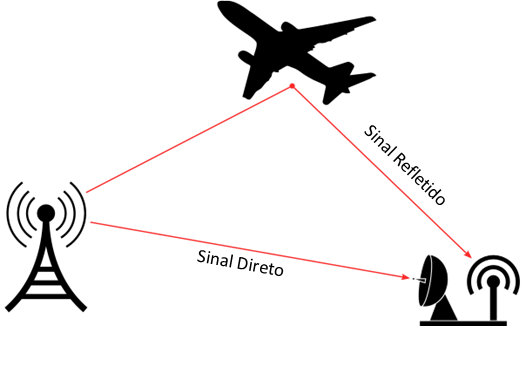
\includegraphics[scale=0.7]{chapters/ch2/assets/esquema_pcl}
\caption[Esquema Geometria Radar Passivo]{Esquema da geometria de um radar passivo}
\label{fig:esquema_pcl}
\end{figure}

O conceito do radar passivo é fazer uma relação cruzada, ou, como mais conhecido o termo, \textit{cross-correlation} entre o sinal direto e o sinal refletido em função das variáveis \textit{delay-time} que pode ser transformado em \textit{bistatic range} e o desvio de \textit{Doppler}. A \textit{cross-correlation}, de forma simples, é uma medida de similaridade entre dois sinais aplicando um atraso num deles, que neste caso, para além do atraso (\textit{delay-time}), também é feita para os diferentes \textit{Doppler}, ou seja, em duas dimensões. No entanto, na prática existem processos analíticos mais eficientes, visto que fazer a \textit{cross-correlation} a duas dimensões em tempo real torna o processo muito pesado computacionalmente.



\subsection{Geometrias Radar}
Podemos classificar os radares quanto à localização dos transmissores e recetores. O ângulo $\beta$ que estes formam, sendo o seu centro o alvo, determina o tipo de geometria \parencite{Baker2019}. Se $\beta <20^{\circ}$, o transmissor e o recetor encontram-se perto ou no mesmo sítio, então estamos perante uma geometria monostática (Figura \ref{fig:monostatic}). Quando o transmissor e recetor estão mais afastados e formam um ângulo com centro no recetor dentro dos seguintes limites, $20^{\circ}<\beta <145^{\circ}$, a geometria é bistática (Figura \ref{fig:bistatic}). Para situações particulares, em que o alvo se encontra a uma cota baixa em relação à linha imaginária que une o transmissor e o recetor ($145^{\circ}<\beta <180^{\circ}$), estamos perante uma geometria \textit{Forward Scatter} (Figura \ref{fig:fsc}).\par   

\begin{figure}[h]
\centering
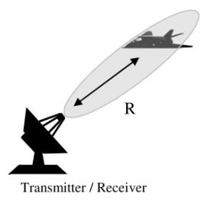
\includegraphics[scale=0.8]{chapters/ch2/assets/monostatic}
\caption[Geometria Monostática]{Geometria Monostática}
\label{fig:monostatic}
\end{figure}

\begin{figure}[h]
\centering
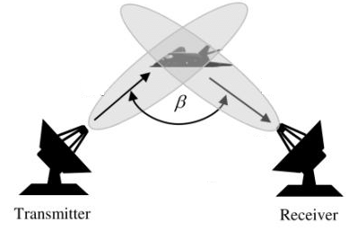
\includegraphics[scale=0.8]{chapters/ch2/assets/bistatic}
\caption[Geometria Bistática]{Geometria Bistática}
\label{fig:bistatic}
\end{figure}

\begin{figure}[h]
\centering
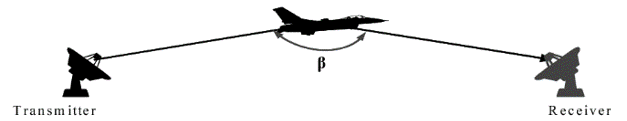
\includegraphics[scale=0.7]{chapters/ch2/assets/fsc}
\caption[Geometria \textit{Forward Scatter}]{Geometria \textit{Forward Scatter}}
\label{fig:fsc}
\end{figure}

Os radares passivos, como já discutido, têm a vantagem de não transmitirem um sinal, e ao invés usar um sinal a ser transmitido por outra fonte. Isto implica que o transmissor e o recetor não estejam no mesmo sítio nem perto, logo, quando se fala em radares passivos, assume-se uma geometria bistática.



\subsection{Alcance Bistático e \textit{Doppler}}
Como falado no ínicio deste capítulo, o alcance bistático, ou \textit{bistatic range} e o desvio de \textit{Doppler} são varáveis fundamentais para qualquer sistema radar e isso não exclui o radar passivo.\par 
O recetor bistático pode medir 3 parâmetros diferentes:
\begin{itemize}
\item A diferença em alcance entre o sinal direto e o sinal que é refletido, ou seja, o \textit{bistatic range};
\item O desvio de \textit{Doppler} do sinal recebido;
\item O ângulo $\theta_{R}$ do sinal recebido, se for usada uma antena de \textit{surveillance }direcional.
\end{itemize}

\subsubsection*{Alcance Bistático} 
Tal como representado na Figura \ref{fig:geom}, tomamos os valores $R_{T}$ como a distância do transmissor ao alvo,  $R_{R}$ como a distância do recetor ao alvo,  $\beta$ como o ângulo entre estes e com centro no alvo, e  $C$ como a distância do transmissor ao recetor, ou, \textit{Baseline}.\par


\begin{figure}[h]
\centering
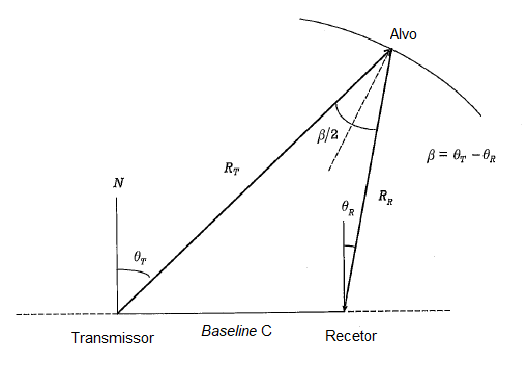
\includegraphics[scale=0.9]{chapters/ch2/assets/geom}
\caption[Parâmetros na geometria bistática]{Parâmetros na geometria bistática}
\label{fig:geom}
\end{figure}

O termo alcance bistático, ou \textit{bistatic range}, é definido em \ref{2.1}. Com este valor é possível criar elipses bistáticas (para duas dimensões) ou elipsoides bistáticos (para três dimensões) com o transmissor e o recetor como dois focos das mesmas. \par

\begin{equation} \label{2.1}
R_{T}+R_{R}-C
\end{equation}

Contudo, se a \textit{baseline} $C$ for um valor conhecido, pode-se extrair o termo \textit{range sum} $R_{T}+R_{R}$. \par
Através do conhecimento do valor de $\theta_{R}$, que é mensurável se a antena de \textit{surveillance} for direcional, a distância do alvo ao recetor é dada pela expressão \ref{2.2}.

\begin{equation} \label{2.2}
R_{R}=\dfrac{\left(  R_{T}+R_{R}\right)^{2}-C^{2}}{2\left(  R_{T}+R_{R}+C sin\theta_{R}\right)}
\end{equation}


Um dos parâmetros importantes quando se fala em alcance bistático é a \textit{range resolution}, ou seja, a resolução em alcance. Este parâmetro é definido pela capacidade de distinguir os alvos que estão muito próximos. Um bom exemplo de um sistema radar que necessite de grande \textit{range resolution} é um sistema de direção de tiro. \par 

Num radar convencional monostático, a resolução em alcance é dada por $\Delta R=c/2B$, onde c é a velocidade de propagação e B a largura de banda do sinal transmitido. No entanto, num radar passivo, a geometria é bistática, o que leva a existirem diferentes elipses bistáticas concêntricas, isto é, com centro no mesmo ponto, o que tem de ser tomado em conta na expressão que representa a \textit{range resolution}:

\begin{equation} \label{2.3}
\Delta r=\dfrac{c}{2B\left( \dfrac{cos\beta}{2}\right)}
\end{equation}

No entanto, este caso é específico para quando os dois alvos estão alinhados relativamente à bissetriz do ângulo $\beta$, como é possivel observar na figura \ref{fig:geom_varios_alvos} o exemplo dos alvos 1 e 2. Para um caso generalizado, como por exemplo o alvo 1 e o alvo 3, a expressão da \textit{bistatic range resolution} (Expressão \ref{2.4}) depende de mais um valor $\varphi$ representado na figura \ref{fig:geom_varios_alvos} como o ângulo entre o seguimento da bissetriz do ângulo $\beta$ e o segmento de reta que une o alvo 1 e o alvo 3 com centro no alvo 1. 

\begin{figure}[h]
\centering
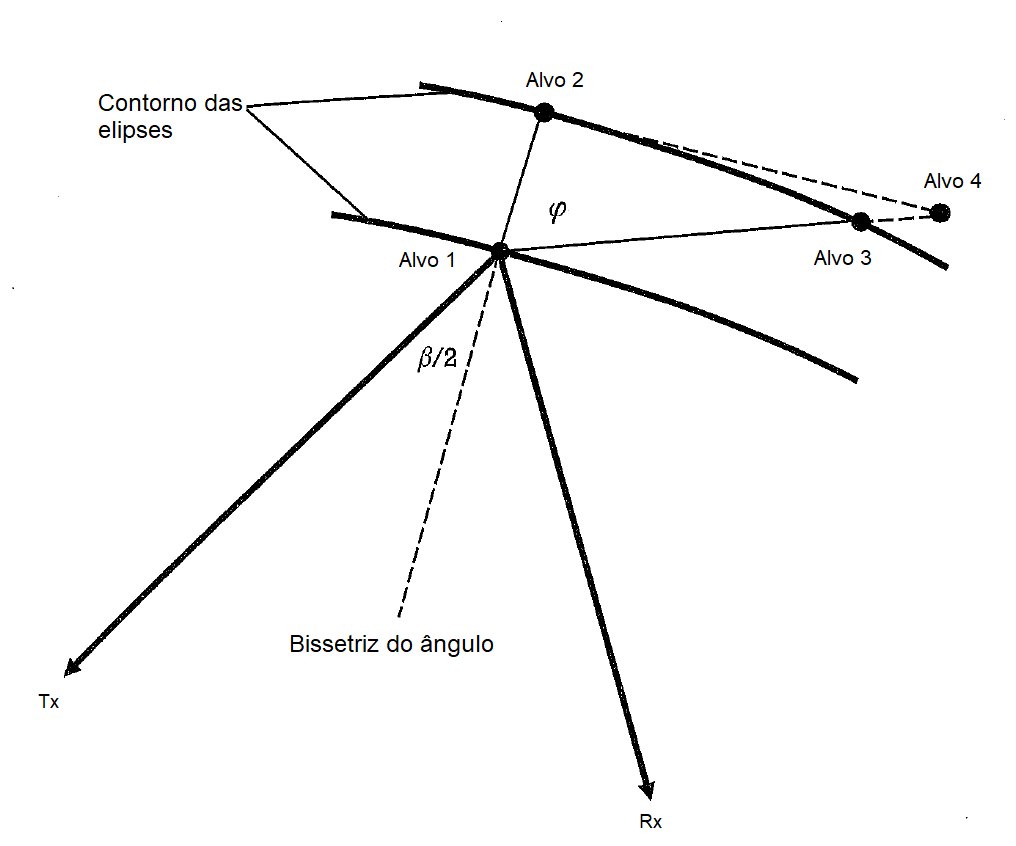
\includegraphics[scale=0.5]{chapters/ch2/assets/geom_varios_alvos}
\caption[Geometria bistática para vários alvos]{Geometria bistática para vários alvos (Adaptada da figura 2.4 \cite{Griffiths2017})}
\label{fig:geom_varios_alvos}
\end{figure}


\begin{equation} \label{2.4}
\Delta r=\dfrac{c}{\left[ 2B\left( \dfrac{cos\beta}{2}\right)\right] cos\varphi}
\end{equation}


A expressão do \textit{bistatic range resolution} permite interpretar a geometria bistática quanto à distância entre o transmissor e recetor. Da expressão \ref{2.4} conclui-se que quanto mais o ângulo $\beta$ se aproxima de um ângulo reto, o denominador tende para um valor próximo de 0, ou seja, a resolução em alcance torna-se fraca. Contudo, nesta situação estamos perante uma geometria \textit{forward scatter}, discutido no inicio deste capítulo, o que pode ser contornando usando vários recetores em locais diferentes.\par 
Para radares passivos, continuando a interpretação da expressão \ref{2.4}, os iluminadores de oportunidade mais utilizados têm pouca largura de banda $B$, o que se reflete numa resolução em alcance mais reduzida. No entanto, os sinais de DVB-T, discutidos no Capítulo \ref{chap:Chapter1}, têm uma largura de banda na ordem dos 8 MHz, o que já permite uma resolução em alcance na ordem dos 40m.

\subsubsection*{\textit{Doppler}} 
Ignorando efeitos relativisticos, o desvio de \textit{Doppler} bistático ocorre quando pelo menos um dos elementos transmissor, alvo, recetor se encontra em movimento. É definido como a taxa de variação temporal do comprimento total do caminho percorrido pelo sinal refletido, normalizado pelo comprimento de onda $\lambda$ \parencite{Willis2005}.  No caso mais comum, em que apenas o alvo se encontra em movimento, o desvio de \textit{Doppler} é dado por \parencite{Willis2005},

\begin{equation} \label{2.5}
f_{D}=\dfrac{2v}{\lambda}cos\delta cos\left( \dfrac{\beta}{2}\right) 
\end{equation}

onde $\delta$ é o ângulo formado pelo sentido do vetor velocidade $v$ e a bissetriz do ângulo $\beta$ com centro no alvo. \par

Na equação \ref{2.5}, quando $\beta =180^{\circ}$, estamos perante uma geometria \textit{forward scatter} e temos um valor de desvio de \textit{Doppler} $f_{D}=0$ para todos os ângulos de $\delta$. Quando $\beta =0^{\circ}$, fica-se reduzido a uma geometria monostática. 


A resolução de \textit{Doppler} no radar bistático é semelhante à resolução de \textit{Doppler} no radar monostático, isto porque depende do tempo de integração $T$ que é um parâmetro escolhido e indiferente à geometria do radar. Quanto maior for o tempo de integração, melhor é a resolução de \textit{Doppler}. A expressão \ref{2.6} define o requisito mínimo entre a separação dos alvos.

\begin{equation} \label{2.6}
\vert f_{a1}-f_{a2}\vert = \dfrac{1}{T}
\end{equation}

sendo que $f_{a1}$ e $f_{a2}$ são os desvios de \textit{Doppler} para cada alvo, definidos em \ref{2.5}. Substituindo as equações dos alvos em \ref{2.5} na equação \ref{2.6}, e resolvendo em ordem a $\Delta v$, ou seja, a diferença entre os dois vetores velocidade projetados na bissetriz do ângulo $\beta$ ($\Delta v=\left( v_{1}cos\delta_{1}-v_{2}cos\delta_{2}\right) $), vem,

\begin{equation} \label{2.7}
\Delta v = \dfrac{\lambda}{2T\cdot cos\left( \beta /2\right) }
\end{equation}

Com esta expressão, assumimos que os alvos partilham a mesma bissetriz, o que na realidade é pouco provável. No entanto, esta restrição pode ser ignorada, se,
\begin{enumerate}
	\item A separação entre os alvos não for suficiente para permitir resolução em \textit{range};
	\item O ângulo entre as bissetrizes dos dois alvos é pequeno.
\end{enumerate}


\subsection{Processamento de Sinal}
Como falado em \ref{contextualização}, o conceito do radar passivo é fazer uma \textit{cross-correlation} entre o sinal direto e o refletido. O problema está no facto de ser computacionalmente muito pesado fazer uma \textit{\gls{2D-CCF}}, sendo necessário a utilização de algoritmos mais eficientes para o cálculo da mesma.\par
O processamento de sinal num radar passivo pode ser, resumidamente, enumerado em oito pontos:
\begin{enumerate}
	\item Receção e reconstrução do sinal direto (\textit{reference signal}$s_{ref}$)
	\item Receção do \textit{surveillance signal} ($s_{r}$))
	\item \textit{Cross-correlation} do $s_{ref}$ e $s_{r}$
	\item Integração de produtos da correlação (FFT)
	\item Filtragem de \textit{clutter}
	\item Deteção de alvos e seguimento no domínio \textit{range/Doppler}
	\item Processamento no plano Cartesiano
	\item Seguimento no plano Cartesiano
\end{enumerate}

\subsubsection*{Equivalência entre um filtro adaptado e \textit{cross-correlation}}

Para \textit{Software Defined Radios}, a implementação de um filtro adaptado pode ser feita através do cálculo de uma \textit{cross-correlation} \parencite{Martorella}. Considerando $s_{0}(t)$ o sinal de saída do filtro adaptado e $h_{MF}(t)$ a resposta do filtro vem, 

\begin{equation} \label{2.8}
s_{0}\left( t\right) =s_{R}\left( t\right)\otimes h_{MF}\left( t\right) =\int s_{R}\left( \tau\right)s_{ref}^{\ast}\left(\tau -t\right)d\tau
\end{equation}

A equação \ref{2.8} mostra que usando um filtro adaptado obtemos um sinal de saída igual ao fazer uma \textit{cross-correlation} entre o $s_{R}$ e $s_{ref}$.\par 

Ao implementar uma \textit{cross-correlation} como mostrado em \ref{2.8}, não se toma em conta o desvio de \textit{Doppler}, visto que se faz a \textit{cross-correlation} apenas numa dimensão. Para se entrar com o desvio de \textit{Doppler} tem de se extender a \gls{2D-CCF},

\begin{equation} \label{2.9}
CCF\left( \tau,\nu\right) =\int s_{R}\left( \tau\right)s_{ref}^{\ast}\left(\tau -t\right)e^{-2\pi j\nu t}d\tau
\end{equation}

onde $\nu$ representa o desvio de \textit{Doppler} que é definido pela \textit{cross-correlation} entre o $s_{R}$ e $s_{ref}$ compensada com o \textit{Doppler shift}.\par
Como o \textit{delay-time} $\tau$ pode ser transformado em \textit{bistatic range}, a \gls{2D-CCF} pode ser representada num \textit{bistatic range-Doppler map}, através da equação \ref{2.10} que representa a \gls{2D-CCF} numéricamente visto que os sinais têm de ser digitalizados com uma certa frequência de amostragem.

\begin{equation} \label{2.10}
CCF\left(l,m\right) =\sum_{n=0}^{N-1} s_{R}\left( n\right)s_{ref}^{\ast}\left(n -l\right)e^{-2\pi j\dfrac{mn}{N}}
\end{equation}

onde $n$ representa o tempo, $l$ o \textit{delay-time}, $m$ o desvio de \textit{Doppler} e $N$ o número total de amostras que depende do \gls{CPI},

\begin{equation} \label{2.11}
N=\dfrac{CPI}{T_{s}}=CPI\cdot F_{s}
\end{equation}

\subsubsection*{Eficiência do cálculo da \gls{2D-CCF}}
De modo a ter um cálculo da \gls{2D-CCF} mais eficiente, há duas condições principais a referir:
\begin{itemize}
\item Cumprir com o teorema de \textit{Nyquist}, ou seja, garantir que a frequência de amostragem é superior ou igual à largura de banda ($F_{s}\geq B$); 
\item Ter um \gls{CPI} longo de forma a obter maior ganho de integração e consequentemente melhor relação sinal-ruído.
\end{itemize}
\par
No entanto, o cálculo de uma \gls{2D-CCF} é computacionalmente muito pesado, e isto pode ser demonstrado com um pequeno exemplo: Para uma largura de banda $B=10MHz$, um $CPI=1s$ e um número de \textit{range bins} e de \textit{doppler bins} igual a 1000 cada, implica um número de multiplicações muito elevado ($10000000\cdot 1\cdot 1000\cdot 1000=10000000000$ cálculos).\par
Para solucionar este problemas existem várias soluções numéricas, como \textit{Correlation FFT}, \textit{Direct FFT} e \textit{Batches Algorithm} \parencite{Martorella}.

\subsubsection*{\textit{Correlation FFT}}
A \textit{Correlation FFT} pode ser obtida através da equação \ref{2.10} mudando o exponencial de posição como representado na eq. \ref{2.12}, de modo a obter uma nova expressão que pode ser calculada como uma \textit{cross-correlation} a uma dimensão com uma compensação de \textit{Doppler}, ou seja, \textit{Doppler bin} ($m$), a \textit{\gls{CCF}} é a \textit{cross-correlation} entre o \textit{reference signal} $S_{ref}$ e o sinal direto com um \textit{Doppler shift}.

\begin{equation} \label{2.12}
CCF\left(l,m\right) =\sum_{n=0}^{N-1} s_{R}\left( n\right)e^{-2\pi j\dfrac{mn}{N}}s_{ref}^{\ast}\left(n -l\right)
\end{equation}

Substituindo $s_{R}\left( n\right)e^{-2\pi j\dfrac{mn}{N}}$ por $s_{R}(n,m)$ vem,

\begin{equation} \label{2.13}
CCF\left(l,m\right) =\sum_{n=0}^{N-1} s_{R}\left( n,m\right) s_{ref}^{\ast}\left(n -l\right)
\end{equation}

Com isto, e sabendo que as \textit{cross-correlations} são calculadas mais eficientemente no domínio de \textit{Fourier}, vem,

\begin{equation} \label{2.14}
CCF\left(l,m\right) = IDFT\left[ S_{R}\left( k,m\right)S_{ref}^{\ast}\left(k\right)\right] 
\end{equation}

com 

\begin{equation} \label{2.15}
S_{R}\left( k,m\right)  = DFT\left[ s_{R}\left( n,m\right) \right] 
\end{equation}

\begin{equation} \label{2.16}
S_{ref}\left( k\right)  = DFT\left[ s_{ref}\left( n\right) \right] 
\end{equation}

A \gls{DFT} da versão do sinal direto com \textit{Doppler shift} pode ser calculada apenas uma vez porque a variável $m$ apenas causa um desvio circular.
Com isto, pode-se tirar algumas conclusões \parencite{Martorella}:
\begin{itemize}
\item Apenas é necessário calcular a \textit{\gls{DFT}} de $s_{R}\left( n,m\right)$ uma vez para $m=0$, visto que para outros valores de $m$ podem ser obtidos com um desvio;
\item Em cada iteração, são calculadas N multiplicações complexas e uma \textit{\gls{IDFT}}.
\end{itemize}

Com isto, concluímos que quanto menos \textit{doppler bins} existirem em relação aos \textit{range bins}, mais eficiente será o cálculo. Este pode ser expressado através da seguinte função de complexidade:

\begin{equation} \label{2.17}
O_{CF}=2Nlog_{2}(N)+N_{f}[N+Nlog_{2}(N)]
\end{equation}

onde,
$N_{f}$: "Número de doppler bins"

\subsubsection*{\textit{Direct FFT}}
Por outro lado, a \textit{Direct FFT} é um método que, tal como a \textit{Correlation FFT} deriva da interpretação da equação \ref{2.10} mas, para cada \textit{time bin} $l$, a \textit{\gls{CCF}} é a \gls{DFT} do produto do sinal recebido com a versão conjugada com \textit{delay} do \textit{reference signal} $S_{ref}$.

\begin{equation} \label{2.18}
CCF\left(l,m\right) = DFT\left[ S_{R}\left( n\right)S_{ref}^{\ast}\left(n-l\right)\right] 
\end{equation}

Da interpretação da equação \ref{2.18} conclui-se que, para cada iteração, são calculadas N multiplicações complexas e u,a \gls{DFT}. A sua função de complexidade pode ser expressa através da expressão \ref{2.19}:


\begin{equation} \label{2.19}
O_{DF}=N_{\tau}[N+Nlog_{2}(N)]
\end{equation}

onde,
$N_{\tau}$: "Número de range bins"

Ao contrário da \textit{correlation FFT}, tal como se pode observar na função de complexidade, a eficiência deste método é dependente do $N_{\tau}$. Isto é, o número de iterações feitas neste método está diretamente relacionado com o número de \textit{range cells}: quanto maior for o número de \textit{range cells} do mapa \textit{range-Doppler}, menos eficiente é este método.\par

\begin{figure}[h]
\centering
\includegraphics[scale=0.6]{chapters/ch2/assets/cfft_vs_dfft}
\caption[Correlation FFT vs Direct FFT]{\textit{Correlation FFT vs Direct FFT} (Figura 2.4 \cite{Martorella})}
\label{fig:cfft_vs_dfft}
\end{figure}

A figura \ref{fig:cfft_vs_dfft} representa de uma forma ilustrativa quando usar a \textit{Direct FFT} ou \textit{Correlation FFT} de acordo com a relação de \textit{Doppler cells} e \textit{range cells} no mapa de \textit{range-Doppler}. Se existirem mais \textit{Doppler cells} a \textit{Direct FFT} é mais eficiente, enquanto se o contrário se verificar, a \textit{Correlation FFT} torna-se mais eficiente.

\subsubsection*{\textit{Batches algorithm}}
Tanto os métodos \textit{direct FFT} e \textit{correlation FFT} são mais eficientes que fazer o cálculo da \gls{2D-CCF}, no entanto, dependem do número de \textit{range} ou \textit{doppler cells} e continuam a ser muito pesadas computacionalmente porque apenas otimizam o cálculo ao longo de uma dimensão.\par 
Apesar de não existir nenhum método perfeito que produza uma solução exata, um método denominado \textit{Batches algorithm} foi proposto e permite otimizar em duas dimensões com uma pequena perda de \textit{\gls{SNR}} reduzindo de forma considerável o peso computacional.\par
O \textit{Batches algorithm} consiste na subdivisão dos dois sinais recebidos, o sinal direto e o sinal refletido no alvo, em segmentos denominados \textit{batches}. Sendo $n_{B}$ o número de \textit{batches} e $N_{B}$ o comprimento do mesmo, com $N=n_{B}\cdot N_{B}$, a expressão da \gls{CCF} é representada pela equação \ref{2.20}.

\begin{equation} \label{2.20}
CCF\left( l,m\right)=\sum_{r=0}^{n_{B}-1}e^{\left( -j2\pi \dfrac{mrN_{B}}{N}\right)}\cdot \sum_{p=0}^{N_{B}-1}s_{R}\left( rN_{B}+p\right)s_{ref}^{\ast}\left( rN_{B}+p-l\right) e^{\left( -j2\pi \dfrac{mp}{N}\right)}   
\end{equation}

Este algoritmo assume que o efeito de \textit{Doppler} é negligenciado dentro de cada \textit{batch}, ou seja, só é calculado para o inicio de cada \textit{batch} $n_{B}$ e assim a equação \ref{2.20} é reduzida à equação \ref{2.21}.

\begin{equation} \label{2.21}
CCF\left( l,m\right)=\sum_{r=0}^{n_{B}-1}e^{\left( -j2\pi \dfrac{mrN_{B}}{N}\right)}\cdot \sum_{p=0}^{N_{B}-1}s_{R}\left( rN_{B}+p\right)s_{ref}^{\ast}\left( rN_{B}+p-l\right)
\end{equation}

A aproximação feita na eq. \ref{2.21} (frequência com que se calcula o desvio de \textit{Doppler}) pode ser representada por uma função \textit{step-wise} em vez de uma função linear (figura \ref{fig:phase_ap}).

\begin{figure}[h]
\centering
\includegraphics[scale=0.6]{chapters/ch2/assets/phase_ap}
\caption[Aproximação de fase]{Aproximação de fase da função de \textit{step} comparada com o ideal: função linear (Figura 2.6 \cite{Martorella})}
\label{fig:phase_ap}
\end{figure}

A equação \ref{2.21} pode ser interpretada de uma forma mais simples (eq. \ref{2.22})ao considerar o somatório do produto entre $s_{R}$ e $s_{R^{\ast}}$ como uma \gls{CCF} e a cada $n_{B}$ é calculado a \gls{DFT} ao longo de $r$.

\begin{equation} \label{2.22}
CCF\left( l,m\right)=\sum_{r=0}^{n_{B}-1}CCF\left( l,r\right) e^{\left( -j2\pi \dfrac{mrN_{B}}{N}\right)}=DFT\left[ CCF\left( l,r\right) \right] 
\end{equation}

Um dos fatores que influencia a eficiência do algoritmo é a escolha da duração dos \textit{batches}. Com isto, é simples concluir que para um determinado intervalo, ao escolher \textit{batches} com maior duração, vai existir um menor número de \textit{batches}, e consequentemente, a \gls{DFT} é calculada ao longo de um menor número de pontos o que vai levar a um menor tempo de processamento. No entanto, ao escolher \textit{batches} com maior duração, vai introduzir um erro maior na aproximação de fase e consequentemente mais perdas em \gls{SNR}.\par
Contudo, \textit{batches} com menor duração implicam o contrário, ou seja, maior número de batches, maior tempo de processamento e menos perdas em \gls{SNR}. \par 
Foi desenvolvido um estudo de grande interesse \parencite{Petri2012} que analisa extensivamente a utilização do \textit{batches algorithm} em que foram recolhidos dados com um radar passivo da \gls{CNIT}. Os resultados da análise da duração dos \textit{batches} com o tempo de processamento e perdas \gls{SNR} encontram-se representados na tabela e figura \ref{fig:bat_snr} respetivamente.\par 

\begin{table}[h]
\centering
\begin{tabular}{@{}ccccc@{}}
\toprule
Comprimento do batch & Tempo de processamento  \\ \midrule
31.28 $\mu s$        & 4.93 $s$                \\
218.76 $\mu s$       & 0.92 $s$                \\
333.29 $\mu s$       & 0.71 $s$                \\ 
924 $\mu s$          & 0.59 $s$                \\ \bottomrule
\label{tab:Tempo de processamento}
\end{tabular}
\caption[\textit{Batches algorithm} - tempo de processamento]{\textit{Batches algorithm} - Análise do tempo de processamento devido ao comprimento dos \textit{batches} (Tabela 2.1 \cite{Martorella})}
\end{table}

\begin{figure}[h]
\centering
\includegraphics[scale=0.5]{chapters/ch2/assets/bat_snr}
\caption[Perdas SNR]{\textit{Batches algorithm} - Análise perdas \gls{SNR} devido ao comprimento dos \textit{batches}(Figura 2.8 \cite{Martorella})}
\label{fig:bat_snr}
\end{figure}


\subsection{Reconstrução do sinal direto}



\subsection{Cancelamento de \textit{clutter}}
No funcionamento do radar passivo, um dos sinais que se quer ter conhecimento é o sinal direto, que é o sinal que é transmitido diretamente do iluminador de oportunidade para o recetor, como representado na figura \ref{fig:esquema_pcl}. Este sinal é submetido a uma atenuação  %de $1/C^{2}$ \parencite{Griffiths2017}, onde $C$ é a \textit{baseline} representada na figura \ref{fig:geom}.
pequena relativamente ao sinal refletido, isto porque a \textit{baseline} $C$ representada na figura \ref{fig:geom} é sempre menor que o \textit{bistatic range}. Logo, o sinal direto pode ser muito mais forte comparado com os ecos dos alvos.\par 
Por mais que se tente fisicamente não receber o sinal direto na antena de \textit{surveillance}, o sinal direto e todas as suas cópias atrasadas no tempo devido a reflexões em objetos e terreno não desejadas (\textit{clutter}) são mais fortes que o sinal refletido no alvo. É possível haver reflexões em edifícios ou algo perto da antena de \textit{surveillance} que possam ser confundidas com o sinal que pretendemos obter, o que pode complicar o cancelamento de todas as réplicas do sinal indesejadas. É de notar, que no caso dos radar \textit{\gls{PCL}}, ou seja, radares passivos, estamos perante uma geometria bistática e isto leva a que o nível de \textit{clutter} na zona da \textit{baseline} possa ser muito forte e ser notável em algumas \textit{range cells}. Este efeito em junção com o sinal direto que possa ser captado na antena de \textit{surveillance} podem dificultar a deteção de alvos.\par 





\subsection{Previsão de \textit{Performance}}



\subsection{Formação de Imagem}


% Chapter 3

\chapter{Teoria de Antenas} % Main chapter title
\label{chap:Chapter3} % For referencing the chapter elsewhere, use \ref{chap:Chapter3} 

%----------------------------------------------------------------------------------------
\section{Teoria Básica de Antenas}
Uma antena é definida como "um dispositivo geralmente metálico (com haste ou fio) para irradiar ou receber ondas de rádio" \parencite{Balanis2016}, ou seja, uma antena, é o dispositivo que permite a transição entre o meio que a rodeia e o equipamento, que se pode observar na Figura \ref{fig:antena transicao}. 
Este dispositivo é um transdutor que converte energia elétrica em ondas eletromagnéticas ou vice versa, sendo que é uma antena de transmissão, se converter um sinal elétrico num sinal eletromagnético e é uma antena de receção, se converter um sinal eletromagnético em sinal elétrico. 

\begin{figure}[h]
\centering
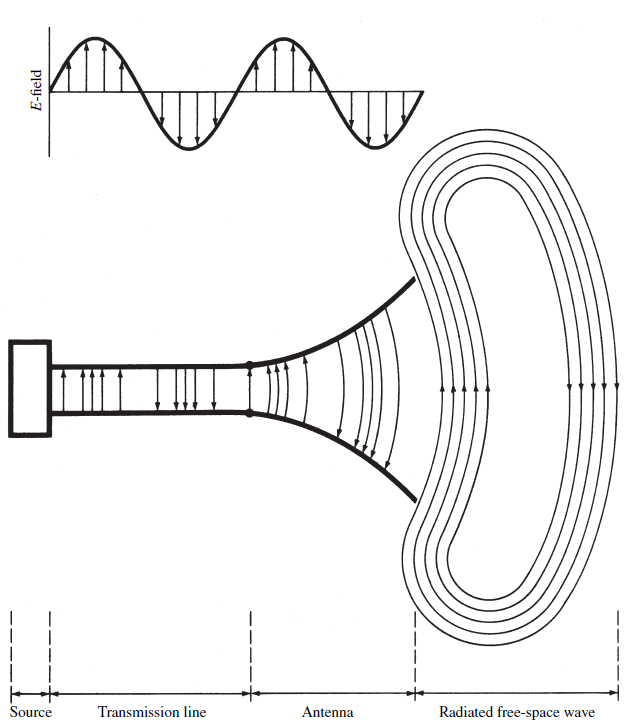
\includegraphics[scale=0.6]{chapters/ch3/assets/Antenna_transicao}
\decoRule
\caption[Antena como meio de transição]{Antena como um meio de transição (Figura 1.1 - \cite{Balanis2016})}
\label{fig:antena transicao}
\end{figure}

\subsection{Tipos de Antenas}
Neste subcapítulo irá ser introduzido de uma forma breve, os vário tipos de antenas, a sua utilização e vantagens entre estes. 

\subsection*{Antenas de Fio}
Estas antenas são umas das mais antigas, que apresentam uma configuração mais simples, como se pode observar na Figura \ref{fig:wire antenna}, sendo apenas constituídas por um fio que pode variar na sua dimensão e na sua forma e ainda podem ser utilizadas nas mais variadas aplicações. Podem tomar uma forma aleatória, desde um fio direito (dipolo) até um fio com as mais diversas formas. \par 
As antenas de fio podem ser encontradas nos mais variados locais, desde aeronaves, carros ou navios a edifícios.

\begin{figure}[h]
\centering
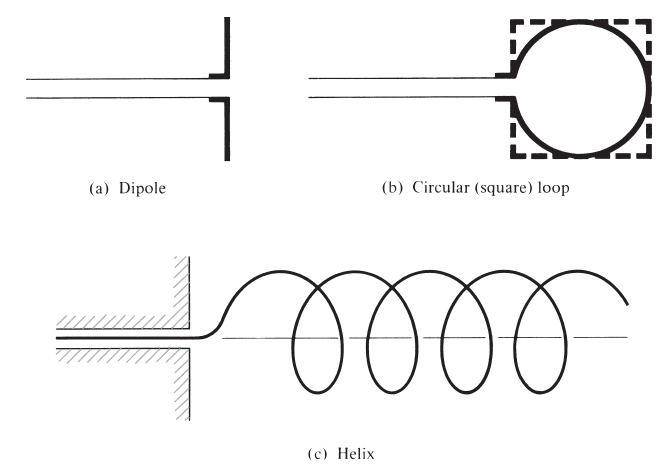
\includegraphics[scale=0.6]{chapters/ch3/assets/wire_antenna}
\decoRule
\caption[Antena de Fio]{Exemplos de vários tipos de antenas de fio (Figura 1.3 - \cite{Balanis2016})}
\label{fig:wire antenna}
\end{figure}

\subsection*{Antenas de Abertura}
Os campos no fim de um guia de ondas aberto não são uniformes devido a esta mesma abertura, assim, para este caso, assume-se que os campos são iguais a como se o guia de ondas continuasse fechado. As antenas de abertura entram quando se pretende aumentar a diretividade à saída do guia, abrindo as extremidades do mesmo de forma a dar uma forma como se observa na Figura \ref{fig:aperture antenna2}. Este tipo de antenas, em especifico as antenas de abertura piramidais, são utilizadas para alimentar ou calibrar grandes antenas de prato.\par
Assim sendo, as antenas de abertura são utilizadas para frequências mais elevadas, especificamente em frequências de micro-ondas e podem ser aplicadas nas mais variadas formas geométricas, como retangulares, elípticas, circulares, piramidais, entre outras.

\begin{figure}[h]
\centering
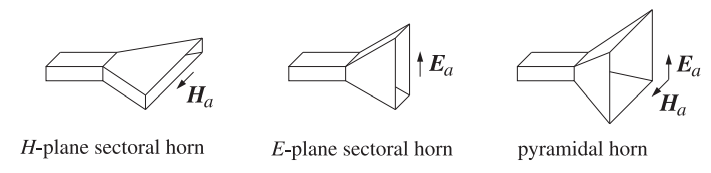
\includegraphics[scale=0.6]{chapters/ch3/assets/aperture_antenna2}
\decoRule
\caption[Antena de Abertura]{Antenas de abertura no plano H, E e piramidal}
\label{fig:aperture antenna2}
\end{figure}


\subsection*{Antenas de \textit{Microstrip}}
Uma antena \textit{microstrip}, conhecida como antena impressa, é um tipo de antena que está inserida numa placa de circuito impresso e funciona como uma antena interna.\par
Hoje em dia são utilizadas em aplicações comerciais, tendo como as suas maiores vantagens o facto de serem baratas e simples de manufaturar e apresentarem um tamanho reduzido. Este tipo de antenas são aplicadas em frequências \gls{UHF}.\par 
A sua construção consiste num \textit{patch} metálico sobre um substrato. Este \textit{patch} pode apresentar as mais variadas formas como representado na Figura \ref{fig:microstrip}, sendo as retangulares e circulares as mais comuns. Têm ainda as vantagens de serem impressas em superfícies com as mais variadas formas, sendo robustas e versáteis nos parâmetros da sua frequência de ressonância, polarização e impedância (\cite{Balanis2016}).

\begin{figure}[h]
\centering
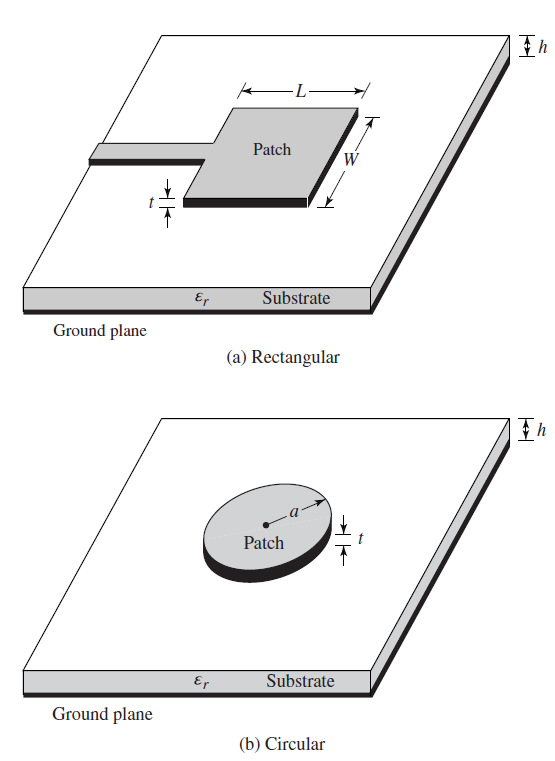
\includegraphics[scale=0.6]{chapters/ch3/assets/microstrip}
\decoRule
\caption[Antena \textit{Microstrip}]{Exemplos de duas configurações de \textit{patches} diferentes (Figura 1.5 - \cite{Balanis2016})}
\label{fig:microstrip}
\end{figure}

\subsection*{Antenas de Matrizes}
As antenas de matrizes surgem nas aplicações em que é necessário mais que um elemento. Consegue-se assim agrupar vários elementos de forma a obter as características pretendidas. Algumas alterações às caraterísticas que se conseguem com este tipo de antenas antenas são o aumento de ganho, alterar o diagrama de radiação, determinar a direção de chegada de um sinal ou maximizar o \gls{SINR}\footnote{\gls{SINR} é um indicador de qualidade de transmissão ajustado a comunicações móveis devido à interferência de outros utilizadores ser mais significativa \parencite{Jeske2004}.}.

\subsection*{Antenas de Lente}
Este tipo de antenas utiliza as propriedades de convergência e divergência das lentes para a receção ou transmissão de sinal. O tamanho da lente a ser utilizada depende da frequência - quanto maior for a frequência, menor a lente. Dito isto, é mais favorável usar este tipo de antenas em frequências mais altas, visto que a lente será menor. As suas aplicações são semelhantes às das refletoras parabólicas, especificamente quando usadas em frequências mais altas e que necessitem de mais largura de banda.

\subsection*{Antenas Refletoras}
As antenas refletoras existem desde o final do século XIX, no entanto começaram a ser aplicadas em radares na Segunda Guerra Mundial e a partir do final do século XX em comunicações espaciais. Estas aplicações devem-se à sua capacidade de transmissões a grandes distâncias. Podem-se apresentar nas mais diversas formas, como plano refletor, refletor curvilíneo, entre outros.\par 
O seu modo de funcionamento baseia-se na convergência da energia numa direção como demonstrado na Figura \ref{fig:reflector}, o que leva, para além de um grande alcance, a uma grande diretividade.

\begin{figure}[h]
\centering
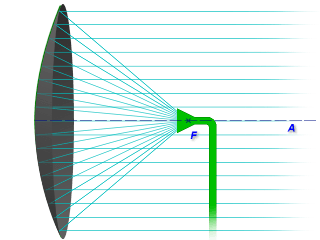
\includegraphics[scale=0.6]{chapters/ch3/assets/reflector}
\decoRule
\caption[Antena Refletora]{Funcionamento de uma Antena Refletora}
\label{fig:reflector}
\end{figure}

\subsection{Parâmetros Fundamentais}
Neste subcapítulo vão ser discutidos os parâmetros mais relevantes que estão relacionados com o funcionamento de uma antena e com a sua \textit{performance}. Grande parte dos parâmetros estão definidos no IEEE 1983 Standard Definitions for Antennas and Propagation.

\subsection*{Diagrama de Radiação}
Um diagrama de radiação é a função ou representação gráfica que descreve as propriedades espaciais de radiação de uma antena. É de extrema importância conhecer este padrão de radiação de uma antena e poder controla-lo, visto que a distribuição de energia eletromagnética, se for mal dimensionada, pode comprometer o projeto. \par 

A manipulação do diagrama de radiação de uma antena é dependente do objetivo da mesma. Podemos ter como finalidade um diagrama de radiação que seja direcional (Figura \ref{fig:direcional}), como numa ligação ponto a ponto, ou podemos como finalidade, um diagrama de radiação omnidirecional (Figura \ref{fig:omnidirecional}), ou seja, que radia, idealmente, com igual intensidade para todas as direções.\par

Para este efeito são utilizadas coordenadas esféricas ($r$, $\varphi$ e $\theta$), sendo que a antena se encontra na origem do referencial. A propriedade mais relevante nos diagramas de radiação é a distribuição espacial, em duas ou três dimensões, da energia radiada em função da posição do observador de acordo com um azimute ($\theta$ constante).\par 

\begin{figure}[h]
\centering
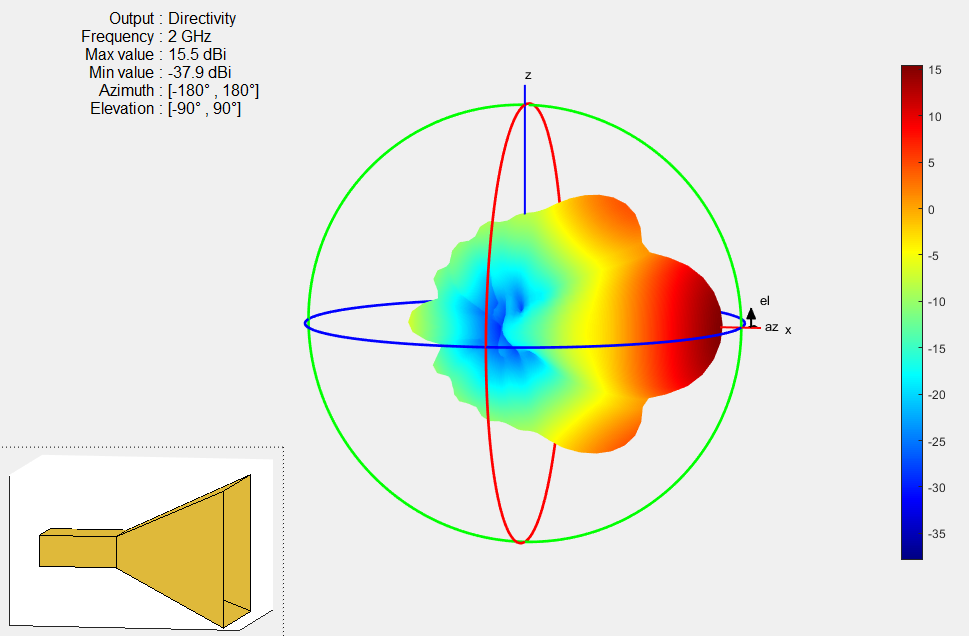
\includegraphics[scale=0.6]{chapters/ch3/assets/matlab_ad1}
\decoRule
\caption[Diagrama de radiação direcional]{Diagrama de radiação direcional - Corneta de guia de ondas dimensionada para 1GHz (MATLAB Antenna Designer Toolkit)}
\label{fig:direcional}
\end{figure}

\begin{figure}[h]
\centering
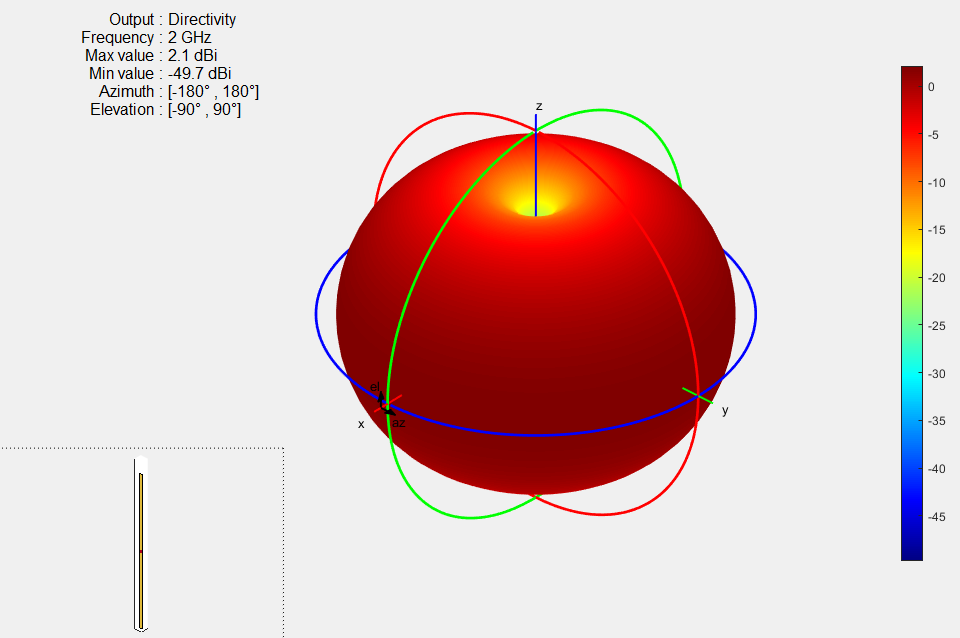
\includegraphics[scale=0.6]{chapters/ch3/assets/matlab_ad2}
\decoRule
\caption[Diagrama de radiação omnidirecional]{Diagrama de radiação omnidirecional - Dipolo dimensionado para 2GHz (MATLAB Antenna Designer Toolkit)}
\label{fig:omnidirecional}
\end{figure}

Os lóbulos são um dos parâmetros fundamentais de um diagrama de radiação, que representam a energia radiada numa direção relativamente ao transmissor e podem ser classificados em lóbulos principais, secundários, laterais e posteriores (Figura \ref{fig:elem_carat_dg}). O lóbulo principal é o lóbulo que contém a direção da radiação máxima, que no caso da Figura \ref{fig:elem_carat_dg}, está definido no sentido do eixo dos zz. Os lóbulos secundários são todos os lóbulos expecto o principal. Os lóbulos laterais são todos os que radiam energia para qualquer direção que não seja a pretendida. Os lóbulos posteriores contêm a energia que é radiada num ângulo de 180$^{\circ}$ em relação à direção do feixe da antena. \par 

A largura de feixe a meia potência (\gls{HPBW}) e a largura de feixe ao primeiro nulo (\gls{FNBW}) estão relacionadas com a capacidade de resolução da antena, ou seja, a sua capacidade de distinguir dois alvos. O critério para distinguir dois alvos é que a \gls{HPBW} seja aproximadamente \gls{FNBW}/2, isto é, se dois alvos estiverem separadas por distâncias angulares iguais ou superiores a \gls{HPBW}$\approx$\gls{FNBW}/2 de uma antena, esta consegue distingui-los \parencite{Kraus1988}. Os fatores que afetam a largura de feixe são o comprimento de onda ($\lambda$), a forma do diagrama de radiação e as dimensões da antena. \par 

\begin{figure}[h]
\centering
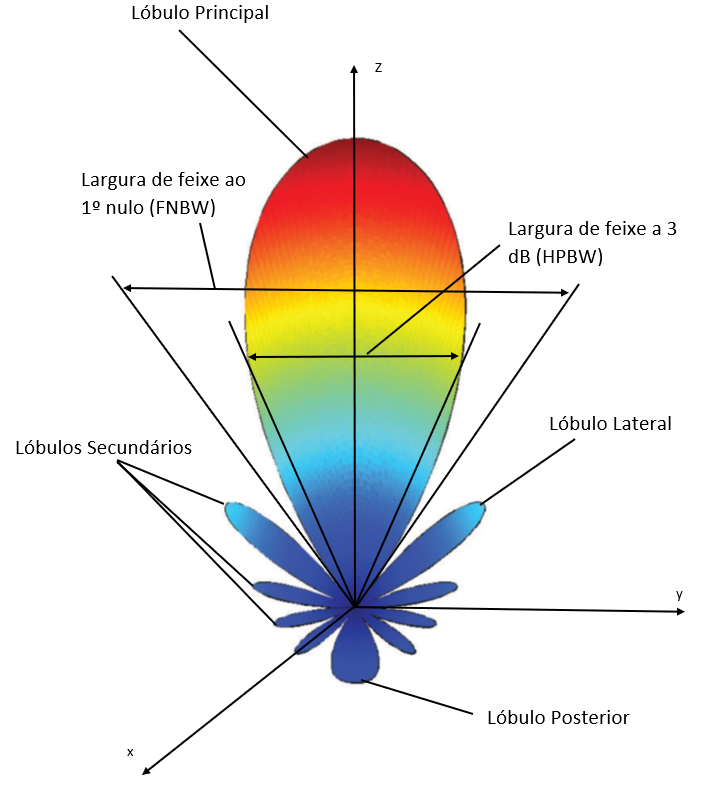
\includegraphics[scale=0.6]{chapters/ch3/assets/elem_carat_dg}
\decoRule
\caption[Elementos caraterísticos do diagrama de radiação]{Elementos caraterísticos do diagrama de radiação}
\label{fig:elem_carat_dg}
\end{figure}

Os diagramas de radiação podem ser classificados quanto à diretividade em que as antenas radiam. Um radiador isotrópico é definido com uma antena hipotética e sem perdas que radia igualmente em todas as direções e é normalmente tomado como referência para exprimir a diretividade de antenas. o radiador direcional é caracterizado por radiar ondas eletromagnéticas em determinadas direções e o radiador omnidirecional radia energia de igual forma em todas as direções \parencite{Balanis2016}.

\subsubsection*{Planos Principais}
Para antenas com polarização linear, discutido com mais detalhe no subcapítulo Polarização, consideram-se os seguintes planos:
\begin{itemize}
\item Plano E: Definido pelo plano que contém o vetor do campo elétrico e a direção da máxima radiação;
\item Plano H: Definido pelo plano que contém o vetor do campo magnético e a direção da máxima radiação.
\end{itemize}
Os eixos do sistemas de coordenadas são escolhidos por forma a que pelo menos um dos planos referido coincidas com os planos do referencial, no entanto, há casos em que pode ser mais favorável escolher outro sistema de coordenadas.


\begin{figure}[h]
\centering
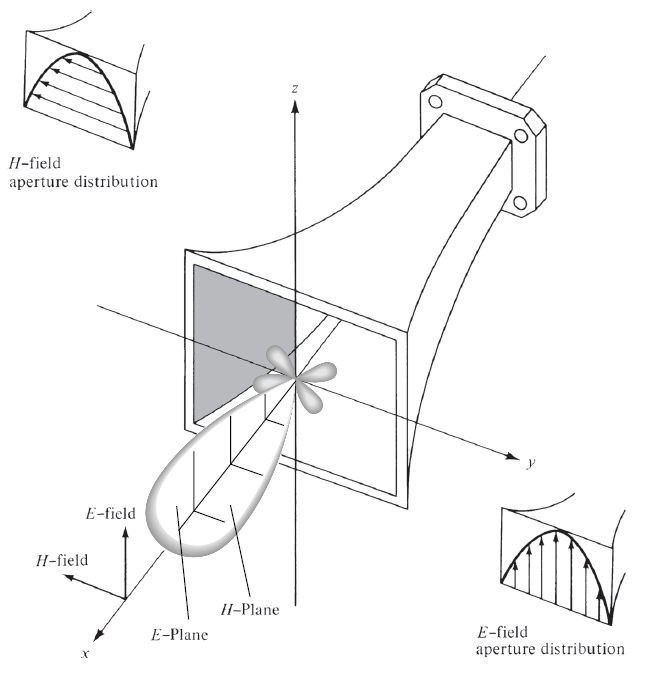
\includegraphics[scale=0.6]{chapters/ch3/assets/campoEH_piramidal}
\decoRule
\caption[Campos E e H de um diagrama de radiação de uma antena]{Campos E e H de um diagrama de radiação de uma antena}
\label{fig:campoEH_piramidal}
\end{figure}

\subsubsection*{Regiões de Campo}
De forma a identificar a estrutura do espaço circundante da antena, este é dividido em três regiões \parencite{Kraus1988}:
\begin{itemize}
\item Região reativa do campo próximo: Definida com a porção do espaço imediatamente em redor da antena, onde predomina o campo reativo;
\item Região do campo próximo (\textit{Região de Fresnel}): Definida como a região da antena entre a região reativa do campo próximo e a região de \textit{Fraunhofer} onde predomina o campo radiado e a sua orientação espacial depende da distância à antena;
\item Região do campo distante (\textit{Região de Fraunhofer}): Caraterizada pela região onde a distribuição angular do campo é maioritariamente independente da distância à antena.
\end{itemize}

Tipicamente, a forma diagrama de radiação é alterado consoante as regiões em que se encontra. Segundo a Figura \ref{fig:alt_tipicas_regioes} presente no artigo \cite{Y.RahmatL.WilliamsR.Yoccarino1995}, o diagrama é mais disperso e uniforme na região reativa do campo próximo. À medida em que a distância à antena aumenta, e que se entra nas regiões de \textit{Fresnel} e \textit{Fraunhofer} a forma do diagrama evidencia mais os seus lóbulos e fica mais regular. A separação entre as regiões reativa do campo próximo e região de \textit{Fresnel} e entre a região de \textit{Fresnel} e região de \textit{Fraunhofer} são definidas pelas expressões \ref{3.1} e \ref{3.2} respetivamente \parencite{Y.RahmatL.WilliamsR.Yoccarino1995}.

\begin{equation} \label{3.1}
R=\dfrac{2L^{2}}{\lambda}
\end{equation}

\begin{equation} \label{3.2}
R=0.62\sqrt{\dfrac{L^{3}}{\lambda}}
\end{equation}

\begin{figure}[h]
\centering
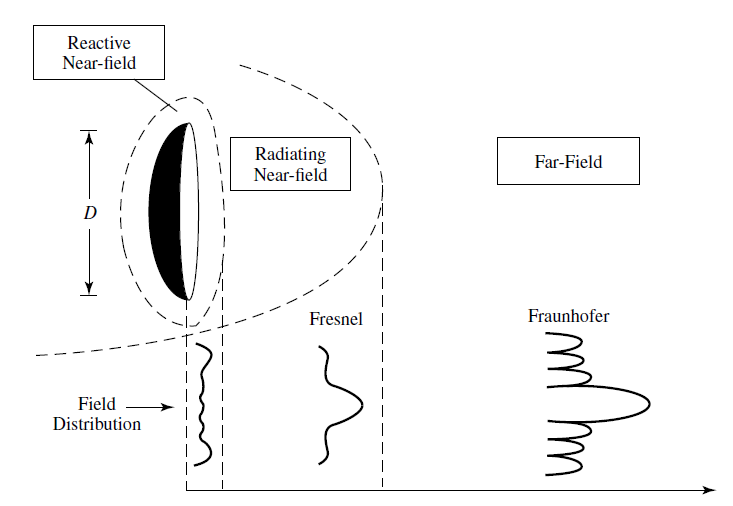
\includegraphics[scale=0.6]{chapters/ch3/assets/alt_tipicas_regioes}
\decoRule
\caption[Alterações típicas da forma do diagrama de radiação]{Alterações típicas do diagrama de radiação desde a reagião reativa do campo próximo à \textit{Região de Fraunhofer}. \parencite{Y.RahmatL.WilliamsR.Yoccarino1995}}
\label{fig:alt_tipicas_regioes}
\end{figure}


\subsection*{Densidade de Potência}

As ondas eletromagnéticas resultam da combinação de um campo magnético e de um campo elétrico que se propaga no espaço. A forma de representar a densidade direcional da quantidade de energia transferida de uma onda eletromagnética é através do vetor de \textit{Poynting}, o qual é definido, contabilizando variações temporais sinusoidais, na equação \ref{3.3}, expressa em \si{\watt\per\meter\squared}.

\begin{equation} \label{3.3}
W_{av}(x,y,z)=\dfrac{1}{2}Re[E\times H^{*}]
\end{equation}

Sendo que o vetor de \textit{Poynting} é uma densidade de potência, ao integrar a componente normal do mesmo, obtém-se na equação \ref{3.4} a potência média radiada pela antena $P_{rad}$ que atravessa uma superfície fechada S.

\begin{equation} \label{3.4}
P_{rad}=P_{av}=\oiint_S W_{rad}\cdot \,ds 
=\dfrac{1}{2} \oiint_S Re[E\times H^{*}]\cdot \,ds
\end{equation}

Como meio de comparação, define-se a potência radiada por um radiador isotrópico na expressão \ref{3.6}, com uma densidade de potência dada por,

\begin{equation} \label{3.5}
W_{0}=\hat{a}_{r}=\hat{a}_{r}\left( \dfrac{P_{rad}}{4\pi r^{2}}\right) 
\end{equation}

\begin{equation} \label{3.6}
P_{rad}=\oiint_S W_{rad}\cdot \,ds 
=\int_{0}^{2\pi}\int_{0}^{\pi}\left[ \hat{a}_{r}W_{0}(r)\right] \cdot \left[ \hat{a}_{r}r^{2}sin\theta \,d\theta \,d\phi \right] = 4\pi r^{2}W_{0}
\end{equation}
 
 
\subsection*{Diretividade}
A diretividade de uma antena é definida com a relação entre a intensidade de radiação numa determinada direção e a intensidade de radiação média em todos as direções. A intensidade média é igual ao quociente entre a potência total radiada pela antena e 4$\pi$ \parencite{IEEE1997}. Sendo que a intensidade de radiação $U$ é obtida pela multiplicação entre a densidade de radiação e o quadrado da distância, a diretividade $D$ de uma antena pode ser descrita pela expressão \ref{3.7}.

\begin{equation} \label{3.7}
D=\dfrac{U}{U_{0}}=\dfrac{4\pi U}{P_{rad}}
\end{equation}

No entanto, para antenas com componentes de polarização ortogonais podem-se definir diferentes diretividades parciais para cada polarização $\theta$ e $\phi$,

\begin{equation} \label{3.8}
D_{0}=D_{\theta}+D_{\phi}
\end{equation}

onde, 

\begin{equation} \label{3.8a}
D_{\theta}=\dfrac{4\pi U_{\theta}}{\left( P_{rad}\right)_{\theta}+\left( P_{rad}\right)_{\phi}}
\end{equation}

\begin{equation} \label{3.8b}
D_{\phi}=\dfrac{4\pi U_{\phi}}{\left( P_{rad}\right)_{\theta}+\left( P_{rad}\right)_{\phi}}
\end{equation}

sendo que o índice $\theta$ e $\phi$ representa a direção que contém as componentes do campo $\theta$ e $\phi$ respetivamente.

Para um radiador isotrópico, a diretividade toma o valor unitário, no entanto, em qualquer outro tipo de radiador, o valor da máxima diretividade irá ser sempre superior a ao valor unitário. Na equação \ref{3.7}, considerando o cálculo para a diretividade máxima, esta pode tomar valores inferiores a 1, o que não acontece na realidade. Com isto, uma expressão mais geral para a diretividade e para a diretividade máxima podem ser definidas na equação \ref{3.9a} e \ref{3.9b} respetivamente.

\begin{equation} \label{3.9a}
D\left( \theta ,\phi\right)=4\pi\dfrac{F\left( \theta ,\phi\right)}{\int^{2\pi}_{0}\int^{\pi}_{0}F\left( \theta ,\phi\right)sin\theta\,d\theta \,d\phi} 
\end{equation}

\begin{equation} \label{3.9b}
D_{0}=4\pi\dfrac{F\left( \theta ,\phi\right)\mid_{max}}{\int^{2\pi}_{0}\int^{\pi}_{0}F\left( \theta ,\phi\right)sin\theta\,d\theta \,d\phi} 
\end{equation}

onde $F\left( \theta ,\phi\right)$ é uma função dos componentes do campo elétrico numa região do campo distante, que, multiplicada por uma constante, resulta a intensidade de radiação.\par 
No entanto, a diretividade máxima também pode ser descrita em função do ângulo sólido de feixe $\Omega_{A}$,\footnote{O ângulo sólido {$\Omega$} é definido como um ângulo tridimensional no centro de uma esfera, que subentende na superfície da mesma uma área medida pelo quadrado do raio da esfera e toma valores adimensionais.}

\begin{equation} \label{3.13}
D_{0}=\dfrac{4\pi}{\dfrac{\left[ \int^{2\pi}_{0}\int^{\pi}_{0}F\left( \theta ,\phi\right) sin\theta\,d\theta \,d\phi\right]}{F\left( \theta ,\phi\right) \mid_{max}} }=\dfrac{4\pi}{\Omega_{A}} 
\end{equation}


\subsection*{Ganho}
A diretividade de uma antena é uma medida que descreve apenas a propriedades direcionais da antena. Por outro lado, o ganho, para além de estar relacionado com a diretividade, também tem em conta a eficiência da antena, discutida mais à frente neste capítulo.\par
O ganho de uma antena é um parâmetro fundamental na \textit{performance} da mesma. Este representa a eficiência em que a antena converte o sinal elétrico em ondas eletromagnéticas, que pode ser definido como ganho absoluto ou ganho relativo. O ganho absoluto de uma antena (definido na equação \ref{3.14}) representa a relação entre a intensidade de radiação radiada numa determinada direção e a intensidade de radiação que chega à antena, se a potência que chega à antena fosse radiada de forma isotrópica. No entanto, a antena isotrópica, como já foi falado neste capítulo, é um caso ideal e não corresponde à realidade. Com isto, utiliza-se o ganho relativo que relaciona a intensidade de radiação radiada de uma antena numa dada direção com a intensidade de radiação radiada a partir de outra antena na mesma direção, denominada antena de referência, quando ambas são alimentadas com a mesma potência de entrada.


\begin{equation} \label{3.14}
G\left( \theta ,\phi\right)=4\pi \dfrac{U\left( \theta ,\phi\right)}{P_{in}}
\end{equation}


Como falado mais à frente neste capítulo, a potência radiada $P_{rad}$ está relacionada com a potência de entrada $P_{in}$ da seguinte forma,

\begin{equation} \label{3.15}
P_{rad}=e_{cd}P_{in}
\end{equation}

sendo que $e_{cd}$ representa a eficiência de radiação da antena. \par 
A partir da equação \ref{3.15}, usando a \ref{3.14}, vem,

\begin{equation} \label{3.16}
G\left( \theta ,\phi\right)=e_{cd} \left[ 4\pi \dfrac{U\left( \theta ,\phi\right)}{P_{rad}}\right] 
\end{equation}

Que está relacionado com a diretividade (equação \ref{3.7}) da seguinte forma,

\begin{equation} \label{3.17}
G\left( \theta ,\phi\right)=e_{cd}D\left( \theta ,\phi\right)
\end{equation}

No entanto, a equação \ref{3.17} não contempla perdas quando o elemento da antena está conectado a um guia, o que provoca perdas indesejadas, através de reflexões. Isto pode ser solucionado com a introdução do termo $e_{r}$ que está relacionado com o coeficiente de reflexão,

\begin{equation} \label{3.18}
e_{r}=\left( 1-\vert\Gamma\vert^{2}\right) 
\end{equation}

Assim sendo, pode-se introduzir o conceito de ganho realizado $G_{re}$ que tem em conta as perdas por reflexão da antena.

\begin{equation} \label{3.19}
G_{re}\left( \theta ,\phi\right)=e_{r}G\left( \theta ,\phi\right)=\left( 1-\vert\Gamma\vert^{2}\right)G\left( \theta ,\phi\right)=e_{r}e_{cd}D\left( \theta ,\phi\right) 
\end{equation}

É de notar, que se a antena for adaptada ao guia, ou seja, se a impedância de entrada for igual à impedância característica ($\vert\Gamma\vert =0$), então, $G=G_{re}$.


\subsection*{Largura de Banda}


\subsection*{Polarização}


\subsection*{Impedância de Entrada}


\subsection*{Eficiência}
\subsubsection*{Eficiência da Antena}
\subsubsection*{Eficiência do Feixe}


\subsection*{Máxima Diretividade e Máxima Área Efetiva}



\subsection*{Equação de Friis e Equação Radar}



\subsection*{\textit{Radar Cross Section}}



\subsection*{Temperatura da Antena}


\subsection*{Síntese}




\section{Simulação de uma Antena}


\subsection{Para Sinais DVB-T}


%% Chapter 4

\chapter{Processamento de Sinal} % Main chapter title
\label{chap:Chapter4} % For referencing the chapter elsewhere, use \ref{chap:Chapter4} 

%----------------------------------------------------------------------------------------

\section{Processamento de Sinal}
Como falado em \ref{contextualização}, o conceito do radar passivo é fazer uma \textit{cross-correlation} entre o sinal direto e o refletido. O problema está no facto de ser computacionalmente muito pesado fazer uma \textit{\gls{2D-CCF}}, sendo necessário a utilização de algoritmos mais eficientes para o cálculo da mesma.\par
O processamento de sinal num radar passivo pode ser, resumidamente, enumerado em oito pontos:
\begin{enumerate}
	\item Receção e reconstrução do sinal direto (\textit{reference signal}$s_{ref}$)
	\item Receção do \textit{surveillance signal} ($s_{r}$))
	\item \textit{Cross-correlation} do $s_{ref}$ e $s_{r}$
	\item Integração de produtos da correlação (FFT)
	\item Filtragem de \textit{clutter}
	\item Deteção de alvos e seguimento no domínio \textit{range/Doppler}
	\item Processamento no plano Cartesiano
	\item Seguimento no plano Cartesiano
\end{enumerate}

\subsubsection*{Equivalência entre um filtro adaptado e \textit{cross-correlation}}

Para \textit{Software Defined Radios}, a implementação de um filtro adaptado pode ser feita através do cálculo de uma \textit{cross-correlation} \parencite{Martorella}. Considerando $s_{0}(t)$ o sinal de saída do filtro adaptado e $h_{MF}(t)$ a resposta do filtro vem, 

\begin{equation} \label{4.1}
s_{0}\left( t\right) =s_{R}\left( t\right)\otimes h_{MF}\left( t\right) =\int s_{R}\left( \tau\right)s_{ref}^{\ast}\left(\tau -t\right)d\tau
\end{equation}

A equação \ref{4.1} mostra que usando um filtro adaptado obtemos um sinal de saída igual ao fazer uma \textit{cross-correlation} entre o $s_{R}$ e $s_{ref}$.\par 

Ao implementar uma \textit{cross-correlation} como mostrado em \ref{4.1}, não se toma em conta o desvio de \textit{Doppler}, visto que se faz a \textit{cross-correlation} apenas numa dimensão. Para se entrar com o desvio de \textit{Doppler} tem de se extender a \gls{2D-CCF},

\begin{equation} \label{4.2}
CCF\left( \tau,\nu\right) =\int s_{R}\left( \tau\right)s_{ref}^{\ast}\left(\tau -t\right)e^{-2\pi j\nu t}d\tau
\end{equation}

onde $\nu$ representa o desvio de \textit{Doppler} que é definido pela \textit{cross-correlation} entre o $s_{R}$ e $s_{ref}$ compensada com o \textit{Doppler shift}.\par
Como o \textit{delay-time} $\tau$ pode ser transformado em \textit{bistatic range}, a \gls{2D-CCF} pode ser representada num \textit{bistatic range-Doppler map}, através da equação \ref{4.3} que representa a \gls{2D-CCF} numéricamente visto que os sinais têm de ser digitalizados com uma certa frequência de amostragem.

\begin{equation} \label{4.3}
CCF\left(l,m\right) =\sum_{n=0}^{N-1} s_{R}\left( n\right)s_{ref}^{\ast}\left(n -l\right)e^{-2\pi j\dfrac{mn}{N}}
\end{equation}

onde $n$ representa o tempo, $l$ o \textit{delay-time}, $m$ o desvio de \textit{Doppler} e $N$ o número total de amostras que depende do \gls{CPI},

\begin{equation} \label{4.4}
N=\dfrac{CPI}{T_{s}}=CPI\cdot F_{s}
\end{equation}

\subsubsection*{Eficiência do cálculo da \gls{2D-CCF}}
De modo a ter um cálculo da \gls{2D-CCF} mais eficiente, há duas condições principais a referir:
\begin{itemize}
\item Cumprir com o teorema de \textit{Nyquist}, ou seja, garantir que a frequência de amostragem é superior ou igual à largura de banda ($F_{s}\geq B$); 
\item Ter um \gls{CPI} longo de forma a obter maior ganho de integração e consequentemente melhor relação sinal-ruído.
\end{itemize}
\par
No entanto, o cálculo de uma \gls{2D-CCF} é computacionalmente muito pesado, e isto pode ser demonstrado com um pequeno exemplo: Para uma largura de banda $B=10MHz$, um $CPI=1s$ e um número de \textit{range bins} e de \textit{doppler bins} igual a 1000 cada, implica um número de multiplicações muito elevado ($10000000\cdot 1\cdot 1000\cdot 1000=10000000000$ cálculos).\par
Para solucionar este problemas existem várias soluções numéricas, como \textit{Correlation FFT}, \textit{Direct FFT} e \textit{Batches Algorithm} \parencite{Martorella}.

\subsubsection*{\textit{Correlation FFT}}
A \textit{Correlation FFT} pode ser obtida através da equação \ref{4.3} mudando o exponencial de posição como representado na eq. \ref{4.5}, de modo a obter uma nova expressão que pode ser calculada como uma \textit{cross-correlation} a uma dimensão com uma compensação de \textit{Doppler}, ou seja, \textit{Doppler bin} ($m$), a \textit{\gls{CCF}} é a \textit{cross-correlation} entre o \textit{reference signal} $S_{ref}$ e o sinal direto com um \textit{Doppler shift}.

\begin{equation} \label{4.5}
CCF\left(l,m\right) =\sum_{n=0}^{N-1} s_{R}\left( n\right)e^{-2\pi j\dfrac{mn}{N}}s_{ref}^{\ast}\left(n -l\right)
\end{equation}

Substituindo $s_{R}\left( n\right)e^{-2\pi j\dfrac{mn}{N}}$ por $s_{R}(n,m)$ vem,

\begin{equation} \label{4.6}
CCF\left(l,m\right) =\sum_{n=0}^{N-1} s_{R}\left( n,m\right) s_{ref}^{\ast}\left(n -l\right)
\end{equation}

Com isto, e sabendo que as \textit{cross-correlations} são calculadas mais eficientemente no domínio de \textit{Fourier}, vem,

\begin{equation} \label{4.7}
CCF\left(l,m\right) = IDFT\left[ S_{R}\left( k,m\right)S_{ref}^{\ast}\left(k\right)\right] 
\end{equation}

com 

\begin{equation} \label{4.8}
S_{R}\left( k,m\right)  = DFT\left[ s_{R}\left( n,m\right) \right] 
\end{equation}

\begin{equation} \label{4.9}
S_{ref}\left( k\right)  = DFT\left[ s_{ref}\left( n\right) \right] 
\end{equation}

A \gls{DFT} da versão do sinal direto com \textit{Doppler shift} pode ser calculada apenas uma vez porque a variável $m$ apenas causa um desvio circular.
Com isto, pode-se tirar algumas conclusões \parencite{Martorella}:
\begin{itemize}
\item Apenas é necessário calcular a \textit{\gls{DFT}} de $s_{R}\left( n,m\right)$ uma vez para $m=0$, visto que para outros valores de $m$ podem ser obtidos com um desvio;
\item Em cada iteração, são calculadas N multiplicações complexas e uma \textit{\gls{IDFT}}.
\end{itemize}

Com isto, concluímos que quanto menos \textit{doppler bins} existirem em relação aos \textit{range bins}, mais eficiente será o cálculo. Este pode ser expressado através da seguinte função de complexidade:

\begin{equation} \label{4.10}
O_{CF}=2Nlog_{2}(N)+N_{f}[N+Nlog_{2}(N)]
\end{equation}

onde,
$N_{f}$: "Número de doppler bins"

\subsubsection*{\textit{Direct FFT}}
Por outro lado, a \textit{Direct FFT} é um método que, tal como a \textit{Correlation FFT} deriva da interpretação da equação \ref{4.3} mas, para cada \textit{time bin} $l$, a \textit{\gls{CCF}} é a \gls{DFT} do produto do sinal recebido com a versão conjugada com \textit{delay} do \textit{reference signal} $S_{ref}$.

\begin{equation} \label{4.11}
CCF\left(l,m\right) = DFT\left[ S_{R}\left( n\right)S_{ref}^{\ast}\left(n-l\right)\right] 
\end{equation}

Da interpretação da equação \ref{4.11} conclui-se que, para cada iteração, são calculadas N multiplicações complexas e u,a \gls{DFT}. A sua função de complexidade pode ser expressa através da expressão \ref{4.12}:


\begin{equation} \label{4.12}
O_{DF}=N_{\tau}[N+Nlog_{2}(N)]
\end{equation}

onde,
$N_{\tau}$: "Número de range bins"

Ao contrário da \textit{correlation FFT}, tal como se pode observar na função de complexidade, a eficiência deste método é dependente do $N_{\tau}$. Isto é, o número de iterações feitas neste método está diretamente relacionado com o número de \textit{range cells}: quanto maior for o número de \textit{range cells} do mapa \textit{range-Doppler}, menos eficiente é este método.\par

\begin{figure}[h]
\centering
\includegraphics[scale=0.6]{chapters/ch4/assets/cfft_vs_dfft}
\caption[Correlation FFT vs Direct FFT]{\textit{Correlation FFT vs Direct FFT} (Figura 2.4 \cite{Martorella})}
\label{fig:cfft_vs_dfft}
\end{figure}

A figura \ref{fig:cfft_vs_dfft} representa de uma forma ilustrativa quando usar a \textit{Direct FFT} ou \textit{Correlation FFT} de acordo com a relação de \textit{Doppler cells} e \textit{range cells} no mapa de \textit{range-Doppler}. Se existirem mais \textit{Doppler cells} a \textit{Direct FFT} é mais eficiente, enquanto se o contrário se verificar, a \textit{Correlation FFT} torna-se mais eficiente.

\subsubsection*{\textit{Batches algorithm}}
Tanto os métodos \textit{direct FFT} e \textit{correlation FFT} são mais eficientes que fazer o cálculo da \gls{2D-CCF}, no entanto, dependem do número de \textit{range} ou \textit{doppler cells} e continuam a ser muito pesadas computacionalmente porque apenas otimizam o cálculo ao longo de uma dimensão.\par 
Apesar de não existir nenhum método perfeito que produza uma solução exata, um método denominado \textit{Batches algorithm} foi proposto e permite otimizar em duas dimensões com uma pequena perda de \textit{\gls{SNR}} reduzindo de forma considerável o peso computacional.\par
O \textit{Batches algorithm} consiste na subdivisão dos dois sinais recebidos, o sinal direto e o sinal refletido no alvo, em segmentos denominados \textit{batches}. Sendo $n_{B}$ o número de \textit{batches} e $N_{B}$ o comprimento do mesmo, com $N=n_{B}\cdot N_{B}$, a expressão da \gls{CCF} é representada pela equação \ref{4.13}.

\begin{equation} \label{4.13}
CCF\left( l,m\right)=\sum_{r=0}^{n_{B}-1}e^{\left( -j2\pi \dfrac{mrN_{B}}{N}\right)}\cdot \sum_{p=0}^{N_{B}-1}s_{R}\left( rN_{B}+p\right)s_{ref}^{\ast}\left( rN_{B}+p-l\right) e^{\left( -j2\pi \dfrac{mp}{N}\right)}   
\end{equation}

Este algoritmo assume que o efeito de \textit{Doppler} é negligenciado dentro de cada \textit{batch}, ou seja, só é calculado para o inicio de cada \textit{batch} $n_{B}$ e assim a equação \ref{4.13} é reduzida à equação \ref{4.14}.

\begin{equation} \label{4.14}
CCF\left( l,m\right)=\sum_{r=0}^{n_{B}-1}e^{\left( -j2\pi \dfrac{mrN_{B}}{N}\right)}\cdot \sum_{p=0}^{N_{B}-1}s_{R}\left( rN_{B}+p\right)s_{ref}^{\ast}\left( rN_{B}+p-l\right)
\end{equation}

A aproximação feita na eq. \ref{4.14} (frequência com que se calcula o desvio de \textit{Doppler}) pode ser representada por uma função \textit{step-wise} em vez de uma função linear (figura \ref{fig:phase_ap}).

\begin{figure}[h]
\centering
\includegraphics[scale=0.6]{chapters/ch4/assets/phase_ap}
\caption[Aproximação de fase]{Aproximação de fase da função de \textit{step} comparada com o ideal: função linear (Figura 2.6 \cite{Martorella})}
\label{fig:phase_ap}
\end{figure}

A equação \ref{4.14} pode ser interpretada de uma forma mais simples (eq. \ref{1.15})ao considerar o somatório do produto entre $s_{R}$ e $s_{R^{\ast}}$ como uma \gls{CCF} e a cada $n_{B}$ é calculado a \gls{DFT} ao longo de $r$.

\begin{equation} \label{4.15}
CCF\left( l,m\right)=\sum_{r=0}^{n_{B}-1}CCF\left( l,r\right) e^{\left( -j2\pi \dfrac{mrN_{B}}{N}\right)}=DFT\left[ CCF\left( l,r\right) \right] 
\end{equation}

Um dos fatores que influencia a eficiência do algoritmo é a escolha da duração dos \textit{batches}. Com isto, é simples concluir que para um determinado intervalo, ao escolher \textit{batches} com maior duração, vai existir um menor número de \textit{batches}, e consequentemente, a \gls{DFT} é calculada ao longo de um menor número de pontos o que vai levar a um menor tempo de processamento. No entanto, ao escolher \textit{batches} com maior duração, vai introduzir um erro maior na aproximação de fase e consequentemente mais perdas em \gls{SNR}.\par
Contudo, \textit{batches} com menor duração implicam o contrário, ou seja, maior número de batches, maior tempo de processamento e menos perdas em \gls{SNR}. \par 
Foi desenvolvido um estudo de grande interesse \parencite{Petri2012} que analisa extensivamente a utilização do \textit{batches algorithm} em que foram recolhidos dados com um radar passivo da \gls{CNIT}. Os resultados da análise da duração dos \textit{batches} com o tempo de processamento e perdas \gls{SNR} encontram-se representados na tabela e figura \ref{fig:bat_snr} respetivamente.\par 

\begin{table}[h]
\centering
\begin{tabular}{@{}ccccc@{}}
\toprule
Comprimento do batch & Tempo de processamento  \\ \midrule
31.28 $\mu s$        & 4.93 $s$                \\
218.76 $\mu s$       & 0.92 $s$                \\
333.29 $\mu s$       & 0.71 $s$                \\ 
924 $\mu s$          & 0.59 $s$                \\ \bottomrule
\label{tab:Tempo de processamento}
\end{tabular}
\caption[\textit{Batches algorithm} - tempo de processamento]{\textit{Batches algorithm} - Análise do tempo de processamento devido ao comprimento dos \textit{batches} (Tabela 2.1 \cite{Martorella})}
\end{table}

\begin{figure}[h]
\centering
\includegraphics[scale=0.5]{chapters/ch4/assets/bat_snr}
\caption[Perdas SNR]{\textit{Batches algorithm} - Análise perdas \gls{SNR} devido ao comprimento dos \textit{batches}(Figura 2.8 \cite{Martorella})}
\label{fig:bat_snr}
\end{figure}



\subsection{Cancelamento de \textit{clutter}}
No funcionamento do radar passivo, um dos sinais que se quer ter conhecimento é o sinal direto, que é o sinal que é transmitido diretamente do iluminador de oportunidade para o recetor, como representado na figura \ref{fig:esquema_pcl}. Este sinal é submetido a uma atenuação  %de $1/C^{2}$ \parencite{Griffiths2017}, onde $C$ é a \textit{baseline} representada na figura \ref{fig:geom}.
pequena relativamente ao sinal refletido, isto porque a \textit{baseline} $C$ representada na figura \ref{fig:geom} é sempre menor que o \textit{bistatic range}. Logo, o sinal direto pode ser muito mais forte comparado com os ecos dos alvos, o que dificulta a deteção de alvos.\par 

\begin{figure}[h]
\centering
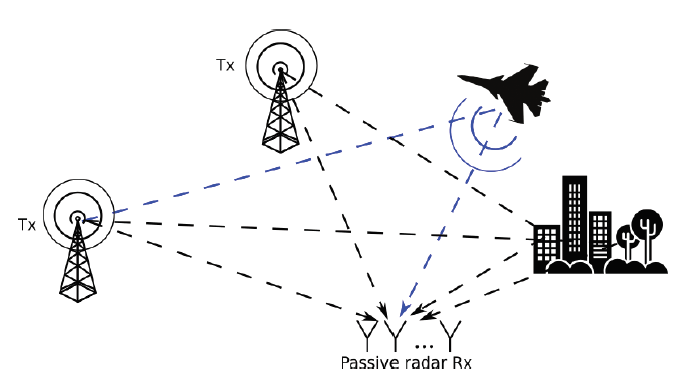
\includegraphics[scale=0.6]{chapters/ch4/assets/clutter}
\caption[Cenário PCL - Clutter]{Cenário PCL - Clutter (Figura 1 \cite{Peto2018})}
\label{fig:clutter}
\end{figure}


Por mais que se tente fisicamente não receber o sinal direto na antena de \textit{surveillance}, este e todas as suas cópias atrasadas no tempo devido a reflexões em objetos e terreno não desejadas (\textit{clutter} representado na figura \ref{fig:clutter}) são mais fortes que o sinal refletido no alvo. É possível haver reflexões em edifícios ou algo perto da antena de \textit{surveillance} que possam ser confundidas com o sinal que pretendemos obter, o que pode complicar o cancelamento de todas as réplicas do sinal indesejadas. É de notar, que no caso dos radar \textit{\gls{PCL}}, ou seja, radares passivos, estamos perante uma geometria bistática e isto leva a que o nível de \textit{clutter} na zona da \textit{baseline} possa ser muito forte e ser notável em algumas \textit{range cells}. Este efeito em junção com o sinal direto que possa ser captado na antena de \textit{surveillance} podem dificultar a deteção de alvos.\par 
O sinal recebido pode ser interpretado de uma forma mais realista como na equação \ref{4.16} para facilitar os processos de cancelamento de \textit{clutter} e identificação das diferentes componentes do sinal.


\begin{equation} \label{4.16}
S_{R}=A_{R}s_{T}\left( t\right)+\sum_{m=1}^{N_{T}}a_{m}s_{T}\left( t-\tau_{T_{m}}\right)e^{\left( 2\pi j f_{D_{m}}t\right)}+\sum_{i=1}^{N_{s}}b_{i}s_{T}\left( t-\tau_{c_{i}}\right)+n\left( t\right)    
\end{equation}

Onde o primeiro termo representa a componente do sinal direto, o segundo termo representa o sinal refletido no alvo, o terceiro termo representa o \textit{clutter} e por fim, o quarto termo representa a componente de ruído.\par

Os aspetos mais importantes na \textit{performance} do cancelamento de \textit{clutter} são a capacidade de operação em tempo real e a eficiência do algoritmo representada no mapa \textit{range-Doppler}. De modo geral, a filtragem, ou cancelamento de \textit{clutter} é feita em dois domínios diferentes: Técnicas de supressão no domínio do espaço para lidar com interferências de alta potência e algoritmos de filtragem de \textit{clutter} no domínio do tempo. Tem sido investigado a aplicação de vários métodos e o artigo \cite{Peto2018} resume a aplicabilidade e comparação de resultados obtidos na utilização dos mesmos tanto como uma explicação sucinta na sua execução.\par 

Existem várias técnicas de cancelamento de \textit{clutter} utilizadas em radares passivos. Os algoritmos de filtragem no domínio do tempo utilizam o \textit{reference signal} de modo a cancelar as réplicas do sinal com um desvio no tempo e de \textit{Doppler} no canal de \textit{surveillance}. Entre estes podemos salientar a aplicação das técnicas de filtragem de \textit{Wiener} com \textit{sample matrix inversion}, \gls{ECA}, \gls{ECA-B}, \gls{ECA-S} \gls{SCA}, \gls{LMS}, \gls{NLMS} e \gls{RLS}.\par

Como jeito de conclusão deste tópico, as figuras \ref{fig:doppler_cancelationtec} e \ref{fig:comp_cost}, retiradas do estudo \cite{Petri2012}  representam a \textit{performance} dos 
vários algoritmos nos dois aspetos mais relevantes, respetivamente no mapa de \textit{range-Doppler} que permite a observação da distorção e resolução do algoritmo e do aumento de \gls{SINR} em relação ao custo computacional  medido em \gls{FLOPS}.


\begin{figure}[h]
\centering
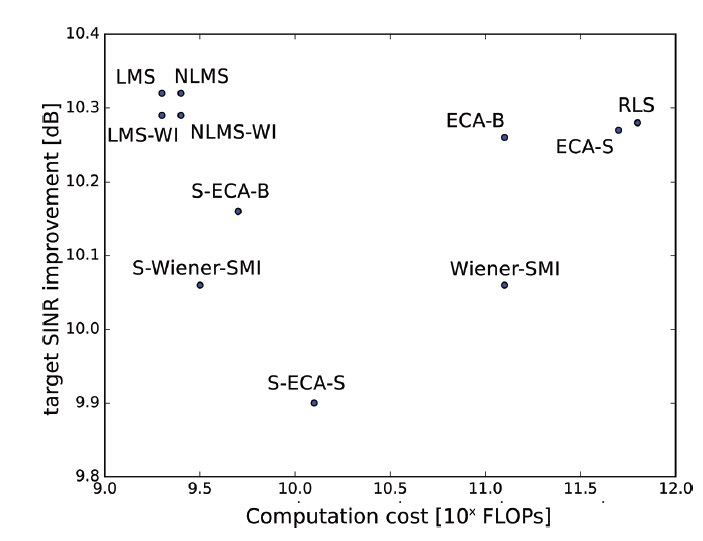
\includegraphics[scale=0.5]{chapters/ch4/assets/comp_cost}
\caption[Mapa da performance dos algoritmos]{Mapa da \textit{performance} dos algoritmos de acordo com o aumento de \gls{SINR} e \textit{computation cost} em \gls{FLOPS} (Figura 16 \cite{Peto2018})}
\label{fig:comp_cost}
\end{figure}

\begin{figure}[h]
\centering
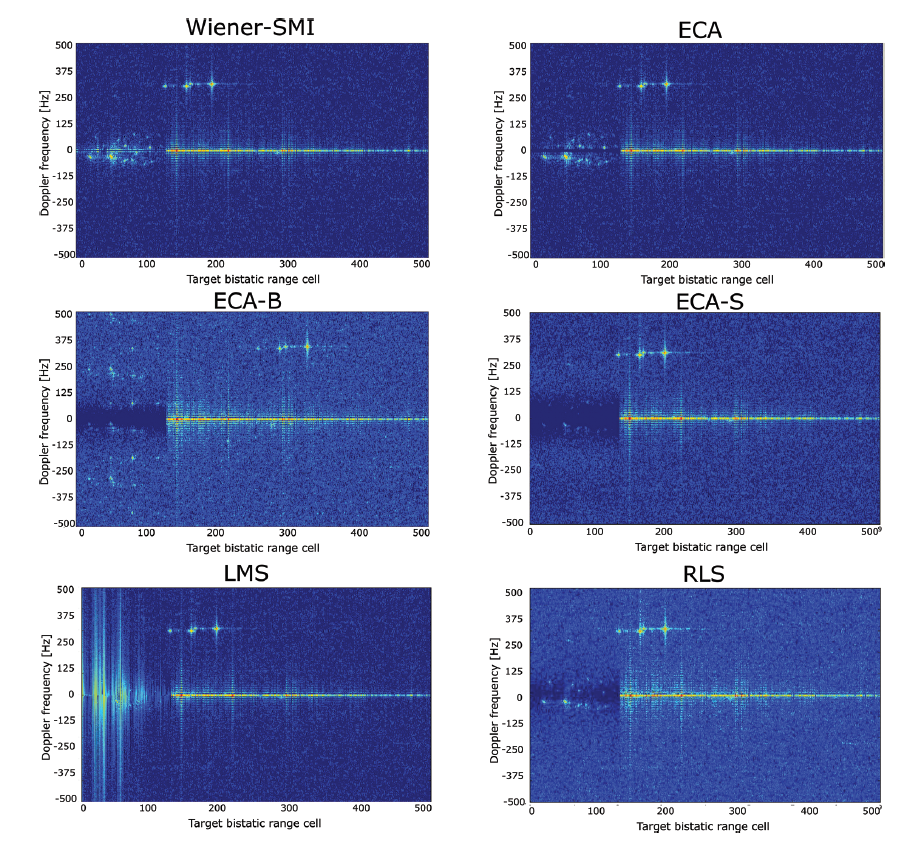
\includegraphics[scale=0.5]{chapters/ch4/assets/doppler_cancelationtec}
\caption[Mapas de range-Doppler dos diferentes algoritmos utilizados]{Mapas de \textit{range-Doppler} dos diferentes algoritmos utilizados (Figura 14 \cite{Peto2018})}
\label{fig:doppler_cancelationtec}
\end{figure}


Destes resultados obtidos, é de realçar o algoritmo \gls{ECA-S} que obteve a melhor \textit{performance} ao custo de um grande \textit{computation cost}. Contudo, pode-se observar os algoritmos do tipo \gls{LMS} e \gls{NLMS}, que apesar de terem um bom aumento de \gls{SINR} com pouco custo computacional, apresentam, como observável na figura \ref{fig:doppler_cancelationtec}, uma grande distorção no mapa \textit{range-Doppler}. Também é de notar, que na figura \ref{fig:comp_cost}, o aumento de \gls{SINR} é pouco relativamente ao custo computacional, isto porque o referencial não está normalizado, ou seja, a janela do eixo das ordenadas toma valores entre $9.8$ e $10.4 dB$ enquanto a janela do eixo das abcissas toma valores entre $10^{9}$ e $10^{12} FLOPS$.


\subsection{Reconstrução e equalização do sinal direto}
Uma das principais diferenças do radar passivo para o radar ativo é que no último o \textit{reference signal} é conhecido visto que é transmitido pelo próprio radar. No caso do radar passivo, a utilização de iluminadores de oportunidade tem como consequências o não conhecimento do sinal direto, visto que para além de receber o mesmo, recebemos as suas réplicas atrasadas no tempo e em \textit{Doppler} e ainda ruído.\par 
De forma a melhorar o sinal direto em quando este é digital, neste subcapítulo vão ser discutidos dois métodos diferentes para a remoção de \textit{multipath} e remoção de picos espúrios formados na função de ambiguidade.

\subsubsection*{Reconstrução do sinal direto} \label{Reconstrução do sinal direto}
Alguns sinais digitais transmitidos, como \gls{DVB-T} em específico, permitem a reconstrução do sinal direto através da desmodulação e re-modulação do sinal direto recebido. Por forma a reconstruir o sinal direto, no caso da \gls{DVB-T}, é importante conhecer o comprimento do símbolo exprimido em amostras, isto porque se a frequência de amostragem do transmissor e do recetor for igual, o comprimento do sinal em amostras é inteiro e a sua receção consiste em meter o sinal no domínio da frequência, usando uma \gls{FFT}. Se este não for o caso, ou seja, que a frequência de amostragem do recetor não seja a definida pelo \textit{standard} \gls{DVB-T}, o comprimento do símbolo não vai ser um número inteiro e a constelação do sinal recebido vai ficar distorcida visto que os pontos depois de usar a \gls{FFT} não vão corresponder às posições de cada subportadora. As soluções para este problema podiam passar por fazer uma nova amostragem do sinal por interpolação, mas isso ia introduzir grandes distorções. Existem várias soluções para este problema, como a utilização de outras transformadas, como a \gls{CZT}.\par 
O próximo passo na receção do sinal \gls{DVB-T} é descodificar os símbolos \gls{OFDM}. Este processo passa por o cálculo inverso no espetro do sinal que foi realizado no transmissor, ou seja, se foi usado uma \gls{FFT} no transmissor, para descodfidicar os símbolos \gls{OFDM} usa-se uma \gls{IFFT}. É de notar que, como falado no parágrafo anterior, se a frequência de amostragem for diferente no transmissor e recetor, a \gls{FFT} que é o mais comum, não pode ser usada. Ao invés, usa-se um método baseado na \gls{CZT}, que não é abordado nesta dissertação, mas pode ser compreendido, tal como todo o processo de reconstrução do sinal direto para radares passivos no estudo \cite{Baczyk2011}.\par 
De seguida, tem-se uma constelação do sinal direto reconstruido como na figura \ref{fig:64QAM} e o próximo passo é a reprodução do sinal no domínio do tempo sem o efeito de \textit{multipath}.

\begin{figure}[h]
\centering
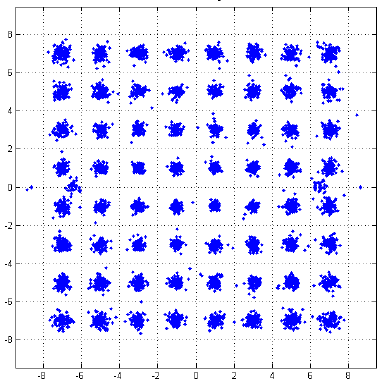
\includegraphics[scale=0.7]{chapters/ch4/assets/64QAM}
\caption[Constelação 64QAM]{Constelação 64QAM (Figura 3.4 \cite{Martorella})}
\label{fig:64QAM}
\end{figure}


\subsubsection*{Equalização do sinal direto}
Em adição à remoção do efeito \textit{multipath} com a reconstrução do sinal direto, é possível equalizar o sinal de forma a remover picos espúrios formados na função de ambiguidade como representados na figura \ref{fig:ACF} relativamente a sinais \gls{DVB-T}.

\begin{figure}[h]
\centering
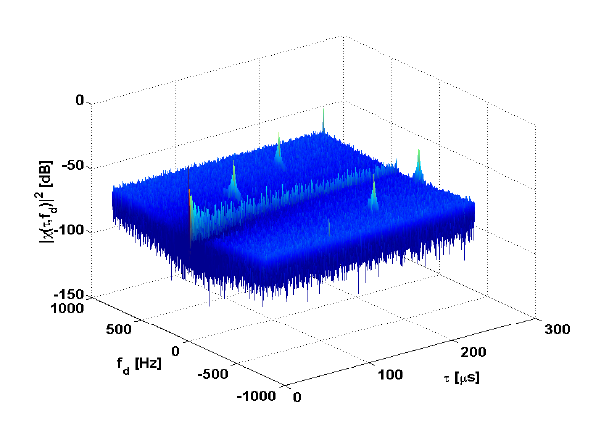
\includegraphics[scale=0.7]{chapters/ch4/assets/ACF}
\caption[Função de ambiguidade - Sinal DVB-T]{Função de ambiguidade - Sinal DVB-T - Presença de picos espúrios (Figura 3.5 \cite{Martorella})}
\label{fig:ACF}
\end{figure}

Um algoritmo eficiente para remover estes picos espúrios passa por estimar tanto para o sinal direto $S_{ref}$ como para um sinal, neste caso \gls{DVB-T}, gerado localmente uma função de \textit{\gls{PSD}} e, equalizar através de uma função de filtragem $H$ que posteriormente, é multiplicada com a transformada do sinal direto $S_{ref}$. De seguida é aplicada a \gls{IFFT} de forma a gerar um sinal direto mais limpo. Um esquema de blocos do algoritmo está representado na figura \ref{fig:equal}.

\begin{figure}[h]
\centering
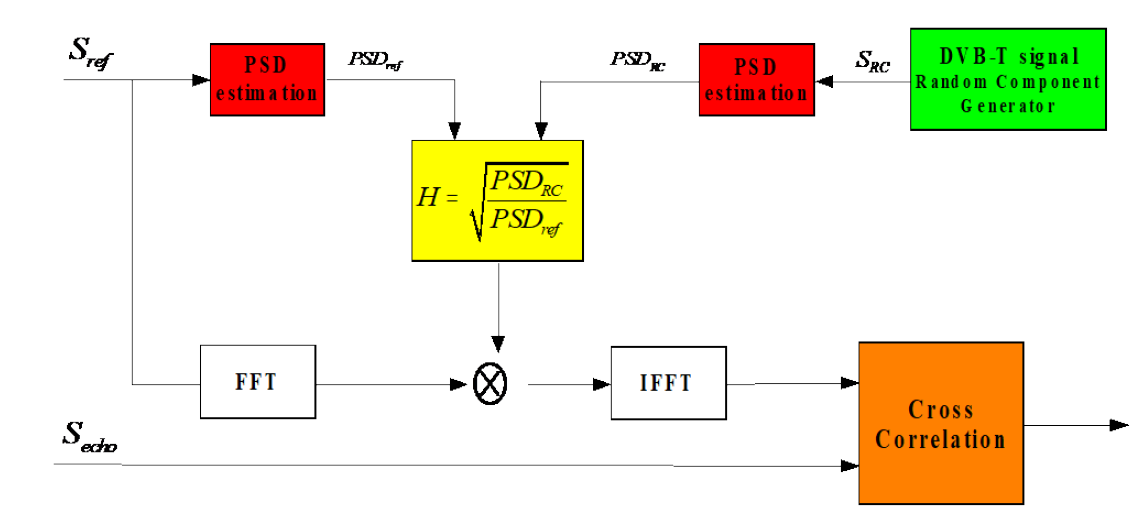
\includegraphics[scale=0.5]{chapters/ch4/assets/equal}
\caption[Diagrama de blocos - Algoritmo de equalização]{Diagrama de blocos - Algoritmo de equalização(Figura 3.6 \cite{Martorella})}
\label{fig:equal}
\end{figure}



\section{Simulação}

\subsection{Função de Ambiguidade}
Uma ferramenta que permite analisar as propriedades do sinal utilizado como iluminador de oportunidade é a função de ambiguidade. Esta função é bidimensional no \textit{time-delay} e em \textit{Doppler}, que representa a distorção devido ao filtro adaptado do recetor, falado no inicio deste capítulo e às propriedades do sinal.\par 
Para um sinal $s(t)$, a sua função de ambiguidade é obtida pela equação \ref{4.17}.

\begin{equation} \label{4.17}
\chi\left( \tau,f\right) =\int s\left( t\right)s^{\ast}\left( t-\tau\right)e^{2\pi jft}dt
\end{equation}

, ou seja, a auto-correlação do sinal recebido.

Utilizando o \textit{matlab} e as ferramentas que este dispõe, é possível calcular funções de ambiguidade de diversos sinais, tendo como um exemplo a figura \ref{fig:ambfun_fmdef} que é resultado do código em anexo \ref{Annex1} apresentado pelo matlab para fazer funções de ambiguidade consoante as caraterísticas do sinal.
\begin{figure}[h]
\centering
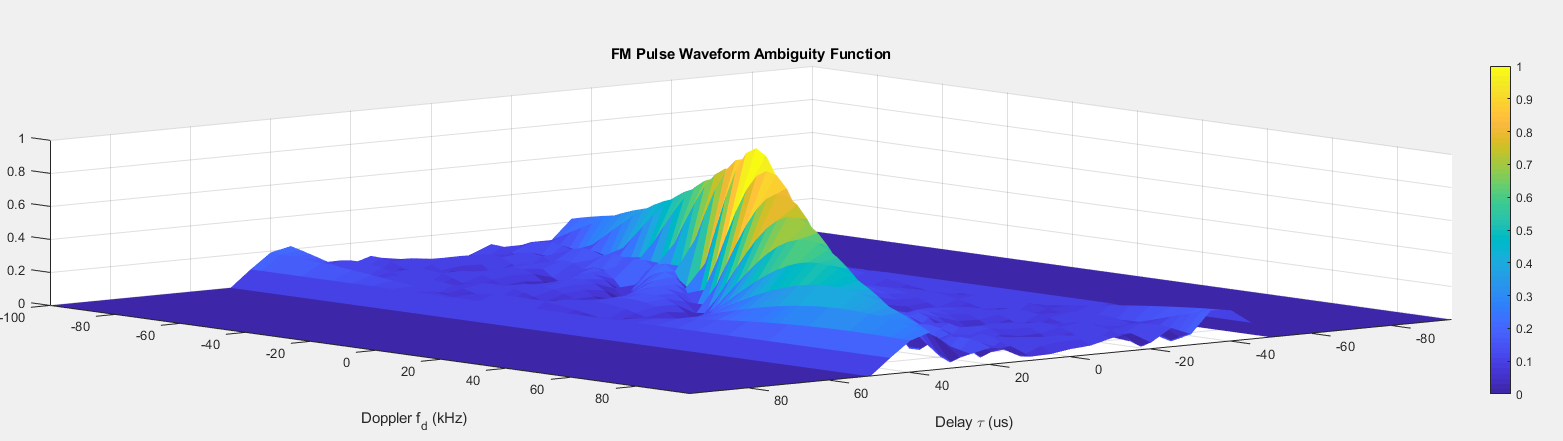
\includegraphics[scale=0.4]{chapters/ch4/assets/ambfun_fmdef}
\caption[Função de ambiguidade para um pulso FM]{Função de ambiguidade para um pulso FM}
\label{fig:ambfun_fmdef}
\end{figure}


\subsubsection{Sinais FM}
Um dos fatores que influencia a performance do sistema é a largura de banda, o que no caso de sinais \gls{FM} é dependente do tipo de música que é transmitido.\par
A figura \ref{fig:ambfun2} é retirada de uma estação a transmitir notícias que corresponde aos gráficos de cima e a transmitir música pop, representado no gráfico de baixo. As principais conclusões que se podem retirar da análise da função de ambiguidade de ambas é que quando é transmitida música, especialmente estilos de músicas como \textit{hard rock}, a largura de banda do sinal transmitido aumenta o que provoca uma função mais estreita e com menor intensidade em redor dos planos de zero \textit{Doppler} e zero \textit{delay}. Consequentemente, este tipo de transmissões permitem uma melhor deteção não só em alcance, como em \textit{Doppler}.

\begin{figure}[h]
\centering
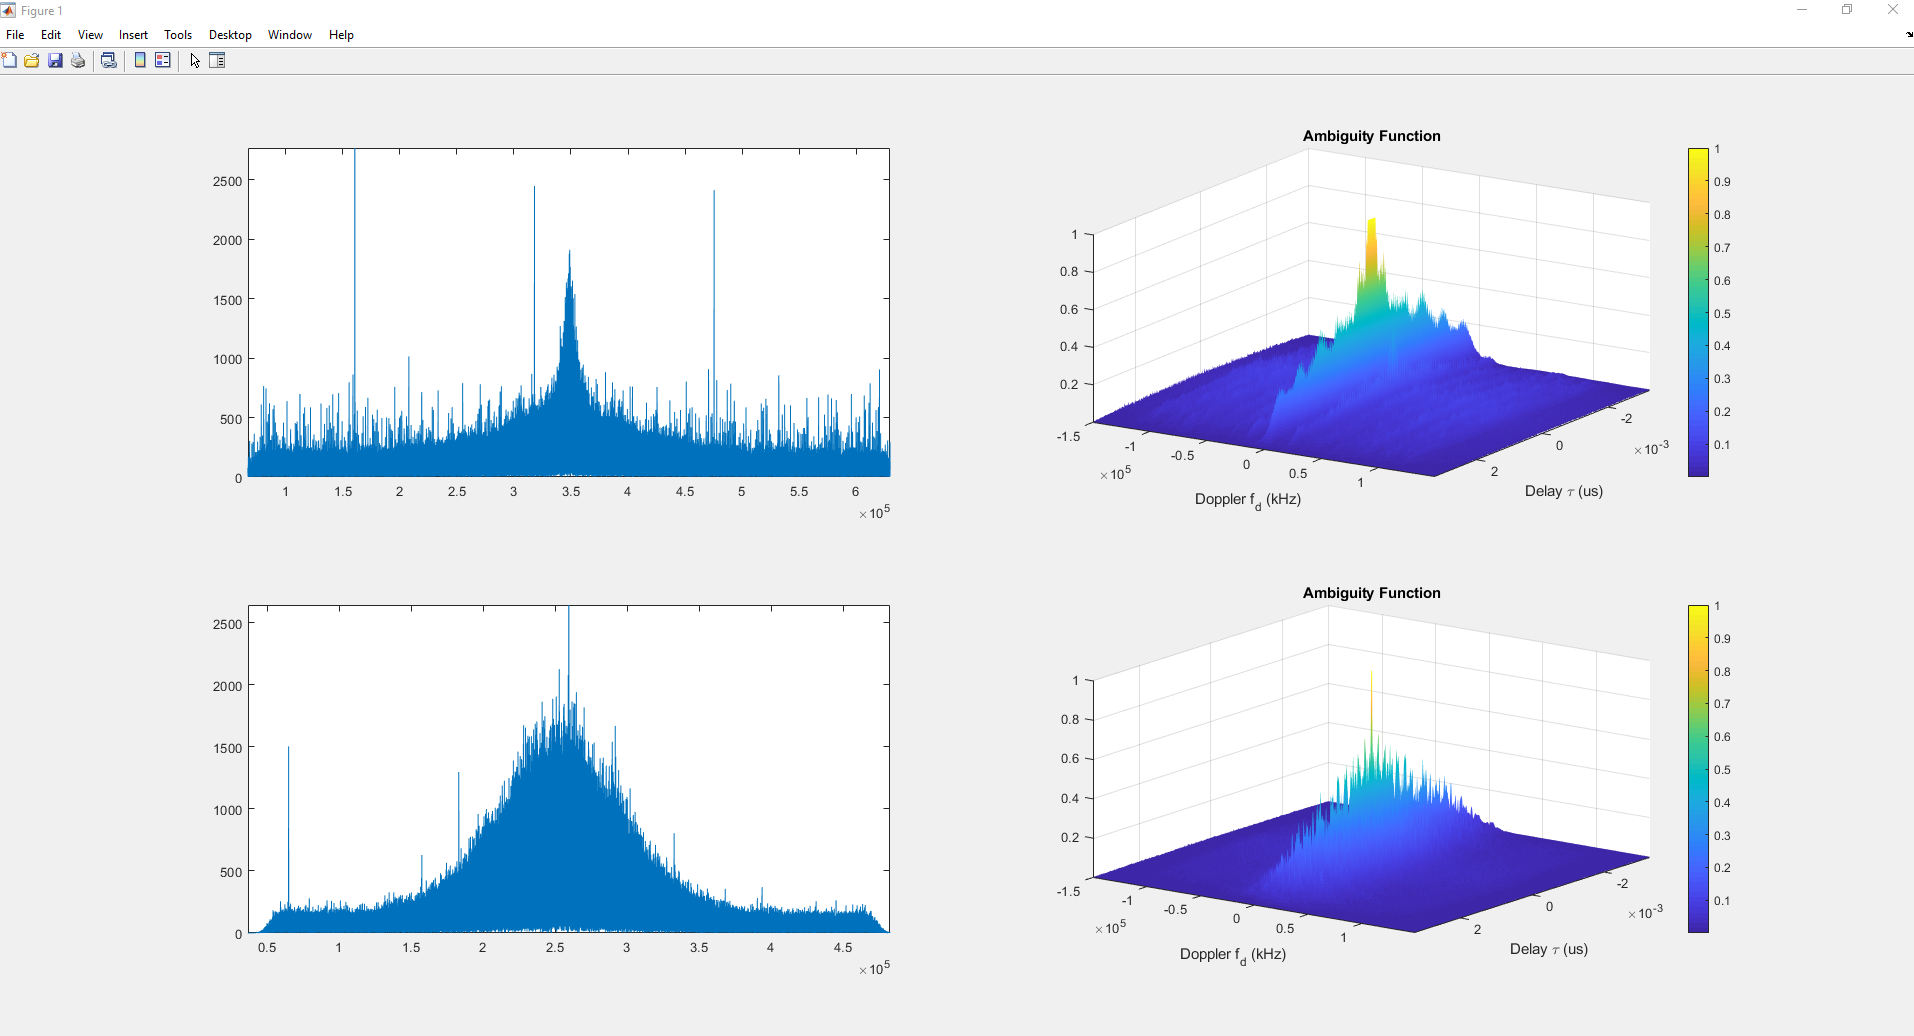
\includegraphics[scale=0.3]{chapters/ch4/assets/ambfun2}
\caption[Função de ambiguidade para uma estação FM]{Função de ambiguidade para um pulso FM retirada de uma estação a dar notícias e música pop}
\label{fig:ambfun2}
\end{figure}
 


\subsubsection{Sinais DVB-T}
Para obter as funções de ambiguidade dos sinais \gls{DVB-T} foi utilizado o LimeSDR com duas antenas de $24 dB$, como descrito no Capítulo \ref{chap:Chapter6}. É de notar que que a antena utilizada no lado direito tem um ganho relativamente superior, o que se deve às fichas que foram cravadas, mas que não tem muito impacto na função de ambiguidade. Dito isto, é mais adequado utilizar este canal para o sinal refletido e o com menor ganho para o sinal direto.\par 

\begin{figure}[h]
\centering
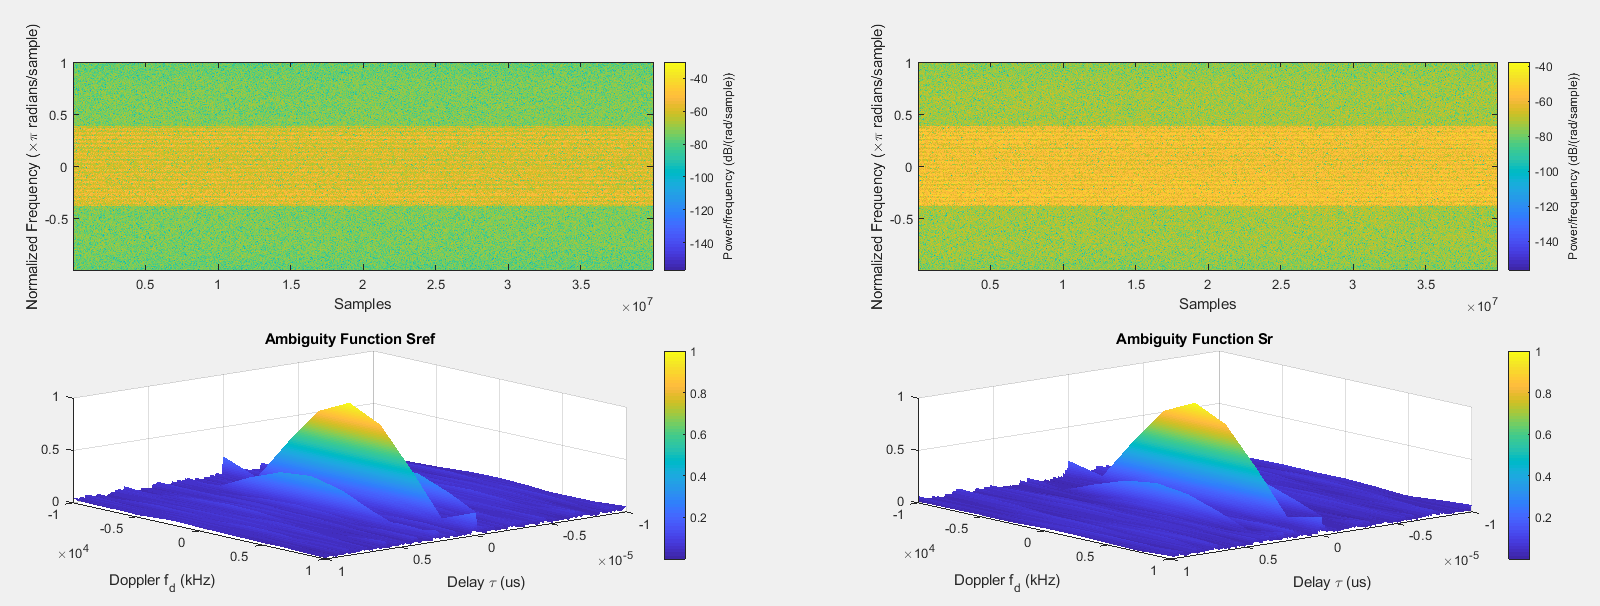
\includegraphics[scale=0.35]{chapters/ch4/assets/dvbt}
\caption[Função de ambiguidade para dois sinais DVB-T]{Função de ambiguidade para dois sinais DVB-T}
\label{fig:dvbt}
\end{figure}
 
Através da equação \ref{4.18}, na frequência $f_{0}=602 MHz$ que é utilizada nesta zona para \gls{DVB-T}, com $c=3x10^{8}m/s$, obtém-se um valor de de variação de frequência de $100Hz$ para $50m/s=180km/h$, ou seja, para uma distância ao alvo com valores inferiores a $15m$, segundo a equação \ref{4.19} para um \textit{delay} de $0.1\times 10^{-6}$, é muito difícil a deteção.

\begin{equation} \label{4.18}
\Delta f=\dfrac{\Delta v}{c}f_{0}
\end{equation}

\begin{equation} \label{4.19}
Range=\dfrac{c\times delay}{2}
\end{equation}









\section{Bases de Dados}

\subsection{Formação de Imagem}
%% Chapter 5

\chapter{Aplicação} % Main chapter title
\label{chap:Chapter5} % For referencing the chapter elsewhere, use \ref{chap:Chapter5} 

%----------------------------------------------------------------------------------------
\section{Sistema Desenvolvido}



\section{Resultados}





%Conclusão - Obrigatória
\begin{conclusion}

%Escreva aqui a conclusão

A conclusão segue-se ao corpo principal dos capítulos que constituem o trabalho, realçando, de forma resumida e nos aspetos mais relevantes, os passos seguidos e os resultados obtidos (mas evitando fazer um resumo que repita aspetos do corpo). Devem expor-se as dificuldades e limitações sentidas, sobretudo se as mesmas limitaram a investigação e prejudicaram o alcançar dos resultados propostos na introdução. 

E, de igual modo, se a investigação desenvolvida mostrou novas vias de trabalho que não puderam ser desenvolvidas, devem evidenciar-se os caminhos que foram abertos, avançando com sugestões e propostas para trabalhos futuros que deem continuidade ao projeto presente.

\end{conclusion}

%----------------------------------------------------------------------------------------
%	BIBLIOGRAFIA
%----------------------------------------------------------------------------------------

\printbibliography[heading=bibintoc]


%----------------------------------------------------------------------------------------
%	APÊNDICES e ANEXOS
%----------------------------------------------------------------------------------------

% Incluir os apêndices da tese como arquivos separados da pasta (appendices)
% Uncomment as linhas para teres à medida que fores criando apendices.

\appendixfile{appendix1}%
%\appendixfile{appendix2}%
%\appendixfile{appendix3}%
%\appendixfile{appendix}%


% Incluir os anexos da tese como arquivos separados da pasta (annexes)
% Uncomment as linhas para teres à medida que fores criando anexos

\annexfile{annex1}%
%\annexfile{annex2}%
%\annexfile{annex3}%


%Imprime no documento os anexos e apendices.
\printappendixes
\printannexes

%----------------------------------------------------------------------------------------

\end{document}
